\documentclass[
	numbers=noenddot, 
	headinclude = true,
	BCOR = 12mm, 
	DIV = 16, 
	twoside
	]{scrbook}
\providecommand*{\Ifstr}{\ifstr}
 
% \usepackage{showframe}
\usepackage{blindtext}
\usepackage{fontspec}
\usepackage{xcolor} 
\usepackage{graphicx}
\usepackage{amsmath} 
\usepackage{bm}
\usepackage{amssymb}
\usepackage{tikz}
\usepackage{tikz-3dplot}
\usepackage{pgfplots}
\usepackage{pgfplotstable}
\usepackage{shellesc}	% Enables the --shell-escape option for tikz externalization.
\usepackage{booktabs}	% Beautiful tables
\usepackage{colortbl}	% Colored rows in tables
\usepackage{enumitem}
\usepackage{eqparbox}
\usepackage{mathtools}
\usepackage{dsfont}
\usepackage{bbding}

% Needed in chapter 3.
\usepgfplotslibrary{groupplots}
\usepgfplotslibrary{colorbrewer}

% For folder tree
\usepackage[newfloat]{minted}
\usemintedstyle{default}
\usepackage{bookmark}
\usepackage{dirtytalk}
\usepackage{dirtree}
\usepackage{listings}
\lstset
{
    language=[LaTeX]TeX,
    breaklines=true,
    basicstyle=\ttfamily\footnotesize,
    keywordstyle=\color{black},
    identifierstyle=\color{hcqblue},
    literate={\\\%}{\%}2
}

\usepackage[labelformat=simple]{subcaption}
\renewcommand\thesubfigure{(\alph{subfigure})}

\usepackage[
	natbib = true,
	defernumbers = true,
	backend = biber,
	maxnames = 10,
	style=ieee,
	doi=false,
	url=false,
	citestyle=numeric-comp,
	sorting=none,
	sortcites,
	giveninits = true,
	dashed = false,
	% eprint = false
]{biblatex} 

\addbibresource{bib-files/examplebib.bib}

% Some header files.
% === Paul Tol's color schemes (https://personal.sron.nl/~pault/) ===%

% Bright qualitative color scheme 
\definecolor{bqblue}{HTML}{4477AA}
\definecolor{bqcyan}{HTML}{66CCEE}
\definecolor{bqgreen}{HTML}{228833}
\definecolor{bqyellow}{HTML}{CCBB44}
\definecolor{bqred}{HTML}{EE6677}
\definecolor{bqpurple}{HTML}{AA3377}
\definecolor{bqgrey}{HTML}{BBBBBB}

\pgfplotscreateplotcyclelist{bright}{
	{bqblue},
	{bqred},
	{bqgreen},
	{bqyellow},
	{bqcyan},
	{bqpurple},
	{bqgrey}
}

% High-contrast color scheme
\definecolor{hcqblue}{HTML}{004488}
\definecolor{hcqyellow}{HTML}{DDAA33}
\definecolor{hcqred}{HTML}{BB5566}
\definecolor{hcqblack}{HTML}{000000}

\pgfplotscreateplotcyclelist{highcontrast}{
	{hcqblue},
	{hcqyellow},
	{hcqred},
	{hcqblack}
}


% Pale qualitative color scheme to fill cells in tables
\definecolor{pqblue}{HTML}{BBCCEE}
\definecolor{pqcyan}{HTML}{CCEEFF}
\definecolor{pqgreen}{HTML}{CCDDAA}
\definecolor{pqyellow}{HTML}{EEEEBB}
\definecolor{pqred}{HTML}{FFCCCC}
\definecolor{pqgrey}{HTML}{DDDDDD}


% More color schemes available at https://personal.sron.nl/~pault/


% === Some beautiful colors stolen from the Stanford identity guide.=== %
% === (https://identity.stanford.edu/design-elements/color/)		===%
\definecolor{stdred}{HTML}{8c1515}
\definecolor{stdsandhill}{HTML}{b3995d}
\definecolor{stdsandstone}{HTML}{d2c295}
\definecolor{stdblack}{HTML}{2e2d29}
\definecolor{stdstone}{HTML}{928b81}
\definecolor{stdredwood}{HTML}{8d3c1e}
\definecolor{stdlagunita}{HTML}{007c92}
\definecolor{stdwarmgrey}{HTML}{3f3c30}
\definecolor{stdcoolgrey}{HTML}{53565A}
\definecolor{stdbrightsandstone}{HTML}{f3efd8}
\definecolor{stdgold}{HTML}{b26f16}
\definecolor{stdpistazie}{HTML}{93C572}
\definecolor{stdspirited}{HTML}{E04F39}
\definecolor{stdspiriteddark}{HTML}{c74632}
\definecolor{stdilluminatingdark}{HTML}{FEC51D}
\definecolor{stdlagunitadark}{HTML}{006b81}
\definecolor{stdskydark}{HTML}{016895}
\definecolor{stdbaydark}{HTML}{417865}
\definecolor{stdpaloverde}{HTML}{279989}
\definecolor{stdpaloverdedark}{HTML}{017e7c}	% Define some colors
%%% layout outer design elements %%% 

% choose main accent colors
\colorlet{accentcolor1}{warmgrey}
\colorlet{accentcolor2}{cardinalred}

% ------------------------------------------------ %
% headline & footline
\usepackage[headsepline=.2pt, ilines]{scrlayer-scrpage}
\pagestyle{scrheadings}
\setkomafont{pagehead}{\small \mainregular \color{accentcolor1}}
% ------------------------------------------------ %

% ------------------------------------------------ %
% declare font families
\newfontfamily{\mainregular}{myriadpro-regular.otf}		% regular sansserif font
\newfontfamily{\mainsemibold}{myriadpro-semibold.otf}	% semibold sansserif font
\setsansfont[UprightFont = *-regular, BoldFont = *-semibold]{myriadpro}

% \newcommand\mainregular{}
% \newcommand\mainsemibold{}
% ------------------------------------------------ %

% ------------------------------------------------ %
% Set fonts and colors for ((sub)sub)sections and paragraphs. 
\addtokomafont{section}{\mainsemibold \Large \color{accentcolor2}}
\addtokomafont{subsection}{\mainregular \large  \color{accentcolor2}}
\addtokomafont{subsubsection}{\mainsemibold \color{accentcolor2}}
\addtokomafont{paragraph}{\mainsemibold  \color{accentcolor2}}
% ------------------------------------------------ %

% ------------------------------------------------ %
% load caption package and specify options
\usepackage[
	format = plain, 
	indention = .5cm, 
	labelsep=endash, 
	textfont = {footnotesize},% , sf}, % remove sf for normal (=serif) font in captions.
	justification = justified, 
	skip = 10pt
	]{caption}

\addtokomafont{captionlabel}{\mainregular \color{accentcolor2}}
\DeclareCaptionFormat{sidebyside}{#1#2\\#3} % Style for figure and caption side by side.
\setlength{\belowcaptionskip}{-0.5\baselineskip}	% Spacing between caption and main text below.	

% Some more options to play around with.
%\captionsetup[sub]{labelfont={blue}}
%\DeclareCaptionFont{blue}{\color{lagunita}}
% \setlength{\abovecaptionskip}{-0.25\baselineskip}	% Spacing between caption and figure above.
% ------------------------------------------------ %


% ------------------------------------------------ %
% Control minimum amount of text on a page
\renewcommand{\floatpagefraction}{.9}
\renewcommand{\topfraction}{.9}
\renewcommand{\bottomfraction}{.9}
\renewcommand{\textfraction}{.1}
% ------------------------------------------------ %


% ================================================ %
% ========Part & Chapter Styles=================== %
% ================================================ %
% ------------------------------------------------ %
% Beginning of part page style 
% Background
\usepackage{graphicx,eso-pic,lipsum,etoolbox}
\providecommand{\chapterhook}{}
\makeatletter
\patchcmd{\scr@startpart}{\thispagestyle}{\chapterhook\thispagestyle}{\typeout{Patching chapter worked OK!}}{\typeout{Patching chapter failed! Oh no!!}}
\newcommand*{\chapterimage}{
	\renewcommand{\chapterhook}{
		\AddToShipoutPictureBG*{% Add picture to background of THIS page only
			\AtPageLowerLeft{%
				% Here, you can add whatever you want for your background image, a TikZ picture, ...
				\begin{tikzpicture}[remember picture,overlay]

				% Uncomment this to get color gradient. 
				\shade [top color=bqyellow,bottom color=bqcyan, middle color = white] (current page.south west) rectangle (current page.north east); 

				% Uncomment this to get monochrome background.
				% \fill[stdsandhill!20] (current page.south west) rectangle (current page.north east);
				\end{tikzpicture}
				
				% Uncomment to use image as background.
				% \includegraphics[width=\paperwidth,height=\paperheight]{example-image-9x16}%
			}%			
		}% Insert image
		\renewcommand{\chapterhook}{}% Restore \parthook
	}%
}
\makeatother

% text
\setkomafont{part}{\mainregular \Huge \color{accentcolor1}}
\setkomafont{partprefix}{\mainsemibold \Huge \color{accentcolor2}}

% put text in lower right corner
\renewcommand*{\partheadstartvskip}{\vspace*{\fill}}% spacing above (maximal)
\renewcommand*{\partheadendvskip}{}% no spacing below
\let\raggedpart\raggedleft%
% End of part page style 
% ------------------------------------------------ %



% ------------------------------------------------ %
% Beginning of chapter style
\setkomafont{chapter}{\mainsemibold \Huge \color{accentcolor2}}
\setkomafont{chapterprefix}{\mainregular \LARGE \color{accentcolor1}}
\newkomafont{chapternumber}{\mainregular \fontsize{70pt}{90pt} \color{accentcolor1}  \selectfont}

\renewcommand\raggedchapter{\raggedleft}

\tikzset{
	headings/base/.style = {
		outer sep = 0pt,
		inner sep = 5pt,
	},
	headings/chapapp/.style = {
		headings/base,
		font = \usekomafont{chapterprefix}
	},
	headings/chapternumber/.style= {
		headings/base,
		font = \usekomafont{chapternumber}
	},
	headings/chapterline/.style = {
		accentcolor1,
		line width = 2pt
	}
}

\makeatletter
\renewcommand*\chapterlinesformat[3]{%
	\Ifstr{#1}{chapter}{%
		\begin{tikzpicture}[baseline=(title.base)]
		\node (title){\parbox[t]{\dimexpr\textwidth-2\pgfkeysvalueof{/pgf/inner xsep}\relax}{\raggedchapter #3}};
		\node[headings/chapapp,anchor=south east] at (title.north east){\Ifstr{#2}{}{}{\chapapp}\strut};
		\useasboundingbox(current bounding box.north west) rectangle ([yshift=-10pt]current bounding box.south east);
		\draw[headings/chapterline] (current bounding box.south east)++(+.5\pgflinewidth,0)--+(0,\paperheight);
		\node[anchor=base west,headings/chapternumber] at([xshift=10pt]title.base-|current bounding box.east){#2};
		\end{tikzpicture}
		\par
	}{%
		\@hangfrom{#2}{#3}% other section levels using style=chapter
	}%
}
\makeatother
% End of chapter style
% ------------------------------------------------ %	% Layout settings: Captions, chapter page, ...
\AtEveryBibitem{% Clean up the bibtex
	 %\clearlist{address}
	 \clearfield{date}
	% \clearfield{eprint}
	 \clearfield{isbn}
	 \clearfield{issn}
	 \clearlist{location}
 	 \clearfield{month}
 	 \clearlist{language}
 	 \clearfield{series}
 }

% Biblatex category for own publications.
\DeclareBibliographyCategory{own}
\addtocategory{own}{BerkeFieldStability}
\addtocategory{own}{berke_transmon_2022}
\addtocategory{own}{CiaranS1}
\addtocategory{own}{hickeyGenericFielddrivenPhenomena2021}

% Biblatex category for `in preparation'
\DeclareBibliographyCategory{prep}
\addtocategory{prep}{inpreparation}

\newbibmacro{string+doiurlisbn}[1]{%
	\iffieldundef{doi}{%
		\iffieldundef{url}{%
			\iffieldundef{isbn}{%
				\iffieldundef{issn}{%
					#1%
				}{%
					\href{http://books.google.com/books?vid=ISSN\thefield{issn}}{#1}%
				}%
			}{%
				\href{http://books.google.com/books?vid=ISBN\thefield{isbn}}{#1}%
			}%
		}{%
			\href{\thefield{url}}{#1}%
		}%
	}{%
		\href{http://dx.doi.org/\thefield{doi}}{#1}%
	}%
}


\DeclareFieldFormat{journaltitle}{#1\isdot}
\DeclareFieldFormat{title}{\usebibmacro{string+doiurlisbn}{\mkbibemph{#1}}}
\DeclareFieldFormat[article,incollection,misc]{title}{\usebibmacro{string+doiurlisbn}{#1}}
\DeclareFieldFormat[thesis]{title}{\usebibmacro{string+doiurlisbn}{\mkbibemph{#1}}}
\DeclareFieldFormat[article,incollection,thesis]{booktitle}{\usebibmacro{string+doiurlisbn}{\mkbibemph{#1}}}
\DeclareFieldFormat[article]{volume}{\addnbspace \textbf{#1}}
\DeclareFieldFormat[article]{number}{\addnbspace \mkbibparens{#1}}
\DeclareFieldFormat[article]{pages}{#1}
\DeclareFieldFormat[incollection]{volume}{\addnbspace Vol.\addnbspace #1}

\renewbibmacro*{journal+issuetitle}{%
	\usebibmacro{journal}%
	\setunit*{\space}%
	\iffieldundef{series}
	{}
	{\newunit
		\printfield{series}%
		\setunit{\addspace}}%
	\usebibmacro{volume+number+eid}%
	\setunit{\addspace}%
	\usebibmacro{issue}%
	\setunit{\addcolon\space}%
	\usebibmacro{issue}%
	\newunit}

\renewbibmacro*{volume+number+eid}{%
	\printfield{volume}%
	\setunit*{\addnbspace}
	\printfield{number}%
	\setunit{\space}%
	\printfield{eid}
}


% If <issue> is a number, map <issue> to <number> and delete <issure> afterwards.
\DeclareSourcemap{
	\maps[datatype=bibtex]{
		\map{
			\step[fieldsource=issue, match=\regexp{\A[0-9]+\Z}, final]
			\step[fieldset=number, origfieldval]
			\step[fieldset=issue, null]
		}
	}
}


% ----------------- Make certain name bold in bibliography -----------------
\def\makenamesetup{%
	\def\bibnamedelima{~}%
	\def\bibnamedelimb{ }%
	\def\bibnamedelimc{ }%
	\def\bibnamedelimd{ }%
	\def\bibnamedelimi{ }%
	\def\bibinitperiod{.}%
	\def\bibinitdelim{~}%
	\def\bibinithyphendelim{.-}}    
\newcommand*{\makename}[2]{\begingroup\makenamesetup\xdef#1{#2}\endgroup}

\newcommand*{\boldname}[3]{%
	\def\lastname{#1}%
	\def\firstname{#2}%
	\def\firstinit{#3}}
\boldname{}{}{}

% Patch new definitions
\renewcommand{\mkbibnamegiven}[1]{%
	\ifboolexpr{ ( test {\ifdefequal{\firstname}{\namepartgiven}} or test {\ifdefequal{\firstinit}{\namepartgiven}} ) and test {\ifdefequal{\lastname}{\namepartfamily}} }
	{\mkbibbold{#1}}{#1}%
}

\renewcommand{\mkbibnamefamily}[1]{%
	\ifboolexpr{ ( test {\ifdefequal{\firstname}{\namepartgiven}} or test {\ifdefequal{\firstinit}{\namepartgiven}} ) and test {\ifdefequal{\lastname}{\namepartfamily}} }
	{\mkbibbold{#1}}{#1}%
}
% ----------------------------------




% Remove day and month.
\AtEveryBibitem{\clearfield{month}}
\AtEveryBibitem{\clearfield{day}}	
% Commands for referencing Chapters, Sections, Subsections, ... 
\newcommand{\chapref}[1]{Chapter~\ref{#1}}
\newcommand{\secref}[1]{Sec.~\ref{#1}}
\newcommand{\refref}[1]{Ref.~\ref{#1}}
\newcommand{\Eqref}[1]{Eq.~\eqref{#1}}
\newcommand{\figref}[1]{Fig.~\ref{#1}}
\newcommand{\appref}[1]{Appendix~\ref{#1}}
\newcommand{\tabref}[1]{Table~\ref{#1}}

% How to write vectors 
\newcommand{\vect}[1]{\textbf{#1}}
\newcommand{\vectgreek}[1]{ {\bm #1} }

% Identity operator
\newcommand{\Id}{\mathds{1}}

% Emphasize command
\newcommand{\highlight}[1]{\emph{#1}}

% Operator
\newcommand{\op}[1]{\hat{#1}}

% Declare signum
\DeclareMathOperator{\sign}{sgn}



% Folder tree structure
\usepackage[edges]{forest}
\definecolor{folderbg}{RGB}{124,166,198}
\definecolor{folderborder}{RGB}{110,144,169}
\newlength\Size
\setlength\Size{4pt}
\tikzset{%
  folder/.pic={%
    \filldraw [draw=folderborder, top color=folderbg!50, bottom color=folderbg] (-1.05*\Size,0.2\Size+5pt) rectangle ++(.75*\Size,-0.2\Size-5pt);
    \filldraw [draw=folderborder, top color=folderbg!50, bottom color=folderbg] (-1.15*\Size,-\Size) rectangle (1.15*\Size,\Size);
  },
  file/.pic={%
    \filldraw [draw=folderborder, top color=folderbg!5, bottom color=folderbg!10] (-\Size,.4*\Size+5pt) coordinate (a) |- (\Size,-1.2*\Size) coordinate (b) -- ++(0,1.6*\Size) coordinate (c) -- ++(-5pt,5pt) coordinate (d) -- cycle (d) |- (c) ;
  },
}
\forestset{%
  declare autowrapped toks={pic me}{},
  pic dir tree/.style={%
    for tree={%
      folder,
      font=\scriptsize\ttfamily,
      grow'=0,
    },
    before typesetting nodes={%
      for tree={%
        edge label+/.option={pic me},
      },
    },
  },
  pic me set/.code n args=2{%
    \forestset{%
      #1/.style={%
        inner xsep=2\Size,
        pic me={pic {#2}},
      }
    }
  },
  pic me set={directory}{folder},
  pic me set={file}{file},
}
\newcommand{\fname}[2]{\begin{tabular}{m{5cm}@{\quad}m{7.5cm}}#1 & \normalfont\footnotesize#2\end{tabular}}
 % Some useful tex commands.

\usepackage{hyperref}
\hypersetup{
	colorlinks=true,
	menucolor = black,
	citecolor = black,
	% urlcolor=stdred,
	urlcolor = stdwarmgrey,
	linkcolor = black
}

% Overwrite \chapter to turn of tikzexternalization of chapter title
\let\oldchapter\chapter		% Store \chapter in \oldchapter
\renewcommand{\chapter}{	%
	\tikzexternaldisable
	\oldchapter%
}

% \widowpenalty10000
% \clubpenalty10000

% For setting paths for tikz/
\usetikzlibrary{external}
\tikzexternalize
\pgfplotsset{compat = 1.18}
\newcommand{\here}{here}

% To control depth of ToC (0 = chapters, 1 = sections, etc)
% \setcounter{tocdepth}{2}

\includeonly{chapters/3_colors/3_colors}
\begin{document}
	
	%%%%%%%%%%%%%%%%%%%% Front part %%%%%%%%%%%%%%%%%%%%
	% frontmatter part (titlepage, abstract, toc) with roman page numbering.
	\frontmatter
	\pagenumbering{roman}
	% \tikzexternaldisable 

	% Note that all chapters are included with \include{} 
	% instead of \input{} such that one can use \includeonly
	% to speed up compilation if desired. \input works as well. 
	\pdfbookmark{Title page}{titlepage}
\begin{titlepage}
\renewcommand{\footnotesize}{\small}
\renewcommand{\footnoterule}{\relax}

\thispagestyle{empty}
\renewcommand{\baselinestretch}{1} 
\begin{center}
	{\vspace*{1mm} \Huge {\color{accentcolor2} \mainregular {Thesis title}} \par}
	{ \Large \vspace*{20mm} {\LARGE \mainsemibold Inaugural-Dissertation} \par \vspace*{4mm} zur \par \vspace*{4mm} Erlangung des Doktorgrades \par \vspace*{4mm} der Mathematisch-Naturwissenschaftlichen Fakultät \par \vspace*{4mm} der Universität zu Köln \par \vspace*{4mm} vorgelegt von \par  \vspace*{15mm}}
	{{\LARGE \mainsemibold Author Name} \par \vspace*{10mm}}
	{\large \vspace*{1ex} aus Birth place \par \vspace*{1ex}}
	% {\vspace*{10mm} {\includegraphics[width=50mm]{auxiliary/logos/LogoUoC_circle}} \vspace*{10mm} \par}
	{\vspace*{10mm} {\includegraphics[width=50mm]{example-grid-100x100pt}} \vspace*{10mm} \par}
	{\large K\"oln 2025}
\end{center}
\end{titlepage}


\thispagestyle{empty}
\begin{center}
\setlength{\tabcolsep}{2em} % horizontal padding
\begin{tabular}{lllll}
	Berichterstatter:           & Prof. Dr. John Doe &  &  &  \\[1em]
	& Prof. Dr. Jane Roe  &  &  &  \\[2em]
	Tag der mündlichen Prüfung: &             &  &  &  \\
	&                        &  &  & 
\end{tabular}
\end{center}

\vfill
Die vorliegende Dissertation wurde von der Mathematisch-Naturwissenschaftlichen Fakult\"at der Universit\"at zu K\"oln angenommen. \emph{\color{lightgray}(only in published version)} \\
\hrule
\vspace{.3cm}
{\noindent \scriptsize Cover illustration: \emph{\color{lightgray} If you're published version has a fancy cover illustration, you might want to explain it here.}}
	\include{auxiliary/abstract}

	\cleardoublepage

	% Add toc to pdfreader content but not to toc.
	\phantomsection
	\pdfbookmark{Table of Content}{toc}
	% Print table of content
	\tableofcontents

	%%%%%%%%%%%%%%%%%%%% Main part %%%%%%%%%%%%%%%%%%%%
	% main part with roman page numbering.
	\mainmatter
	\pagenumbering{arabic}

	\addchap{Outline} 	% Use \addchap{} instead of \chapter*{} to get a bookmark in the pdfreader.

This thesis applies concepts from the theory of \highlight{many-body localization} (MBL) to the \highlight{transmon} platform for quantum computing to scrutinize prevalent processor architectures for the emergence of \highlight{quantum chaotic} behavior. In detail, this work is organized as follows: 

\textbf{Chapter 1} intends to give readers without prior knowledge of quantum computing a brief outline of the subject. It positions the transmon in the zoo of possible qubit platforms and discusses its leading role in the current NISQ era. We introduce some frequently used basic vocabulary. Following this, \textbf{Chapter 2} acquaints with the concepts of many-body localization and quantum chaos. 
\blindtext

These chapters are further supplemented by three appendices, providing examples of state-of-the-art transmon processors, additional results, and an extended discussion of some of the more technical aspects of this work, including details on the implementation.

Last mentioned, ...	% Chapter without number in ToC
	\graphicspath{{chapters/1_basicfeatures/figures/}}

\chapter{Basic features of the template}
To compile the thesis, generate the bibliography, and ensure flawless cross-references between the table of contents, main text, citations, and bibliography, run
\begin{lstlisting}
lualatex main_thesis.tex
biber main_thesis
lualatex main_thesis.tex
lualatex main_thesis.tex
\end{lstlisting}
Of course, running these four commands manually every time is unnecessary. All \LaTeX editors I ever used (Sublime Text, VS Code, TeXstudio, TeXmaker, TeXShop, and Overleaf), allow you to set \verb|lualatex| as the default compiler and \verb|biber| as the bibliography processor. Additionally, all these editors enable you to define this sequence of commands as the standard build process, so your document is compiled correctly with a single action.

\paragraph{Why lualatex?} 
This template uses \verb|lualatex| instead of \verb|pdflatex| for two main reasons:
(i) Font Management: The template relies on the \verb|fontspec| package to handle different font types (e.g., sans-serif for captions and serif for the main text), which requires lualatex for compilation.
(ii) Memory Management: lualatex has a superior memory allocation system that dynamically adjusts as needed. This is particularly important when creating figures in \LaTeX with TikZ/pgfplots, where even simple 2D surface plots can lead to out-of-memory errors with \verb|pdflatex|.

Beyond these two reasons, \verb|lualatex| offers several other advantages, such as powerful Lua scripting capabilities. If you're interested, you can find numerous discussions on the benefits of \verb|lualatex| on \href{tex.stackexchange.com}{TeX Stack Exchange}.

\paragraph{Why biber and biblatex?}

This template uses \verb|biblatex| with the \verb|biber| backend instead of \verb|bibtex|. \verb|Biblatex| is more modern and versatile, and there’s virtually no reason to prefer \verb|bibtex| over \verb|biblatex|. The continued popularity of \verb|bibtex| is likely due to (bad) habit, both among users and some journals that still mandate its use.

For a thesis with a straightforward bibliography, \verb|bibtex| might be sufficient. However, \verb|biblatex| makes customization easier. Moreover, for more complex bibliography structures---such as our CRC183 project, which involves multiple independent bibliographies, cross-references between them, chapter-specific citation highlighting, and automatic correction of incorrect entries---\verb|bibtex| would have been completely inadequate.
See \chapref{chap:biblatex} for details.



\section{Documentclass}
This template is built on the \href{https://ctan.org/pkg/koma-script?lang=de}{KOMA-script} class \verb|scrbook|. Whether to use the standard \verb|book| class or its KOMA-Script counterpart is largely a matter of personal preference. The KOMA-Script bundle is widely recognized as an excellent package, and personally, I find \verb|scrbook| easier to customize while also preferring its default layout.

The document class is loaded with the following options:
\begin{lstlisting}
\documentclass[numbers=noenddot, headinclude = true,
	BCOR = 12mm, DIV = 16, twoside]{scrbook}
\end{lstlisting}
Below is an explanation of some of these options.

\subsection{Page layout without the \texttt{geometry} package}
One of the key strengths of the KOMA-Script classes is their built-in handling of type area and other typographic settings. The package author has extensive expertise in typography and has incorporated many best practices directly into its implementation. The KOMA-Script manual states:
 \say{Various algorithms and heuristic methods for constructing an appropriate type area have been discussed in the literature. These rules are known as the `canons of page construction.' [\ldots] The result is that the aspect ratio of the type area corresponds to the proportions of the page. [\ldots] In a two-sided document (e.g. a book), however, the entire inner margin (the margin at the spine) should be the same size as each of the two outer margins.}

The scrbook class automatically generates margins that conform to these typographic principles. The DIV parameter controls the type area width: the larger the value, the smaller the margins. The underlying construction mechanism is explained in Section 2.2 of the KOMA-Script manual, particularly in Figure 2.1.

Furthermore, \verb|headinclude=true| ensures that the header is included in the type area calculations as part of the text, and \verb|BCOR=12mm| adds a binding correction to the inner margin.

The KOMA-Script eliminates the need for the \verb|geometry| package that is otherwise often used to adjust margins. Manually setting margins can unintentionally violate typographic rules, potentially leading to poor readability. As the KOMA-Script manual warns:

\say{The practice of doing things oneself has long been widespread, but the results are often dubious because amateur typographers do not see what is wrong and cannot know what is important. This is how you get used to incorrect and poor typography. [...] Now, the objection could be made that typography is a matter of taste. When it comes to decoration, one could perhaps accept that argument, but since typography is primarily about information, not only can mistakes irritate, but they may even cause damage.}
(I recommend everyone to read Sec.~2.X of the manual, I enjoyed its polemic tone)

\paragraph{A confession} After emphasizing the importance of adhering to typographic best practices, I must confess: this template violates them.

For each combination of font size, font type (serif vs. sans-serif), and paper size, there is an optimal maximum number of characters per line to ensure readability. This determines the highest recommended \verb|DIV| value. The template uses \verb|DIV=16|, which exceeds the recommended value. As a result, LaTeX issues a \verb|Bad type area settings!| warning and suggests decreasing the \verb|DIV| value.
However, I deliberately chose smaller margins because I personally prefer this layout. My poor justification is that the recommended maximum character count per line is intended for inexperienced readers, whereas academic writing assumes a more advanced audience accustomed to dense text.



\section{Structure of the thesis}

According to the \href{https://mathnat.uni-koeln.de/sites/dekanat/official/Ordnungen/Promotionsordnung_2020.pdf}{`Promotionsordnung der math.-nat. Fakultät (2020)'} (PO2020), a Ph.D. thesis must include
\begin{itemize}
	\item a cover / title page,
	\item an abstract (PO2020 specifies that an English abstract is sufficient; a German version is not required),
	\item several chapters including an introduction, presentation of results, and discussion,
	\item the closing statement from §7 Absatz 8, PO2020, along with a list of your publications.
\end{itemize}
It is also common to include a thesis outline and acknowledgments. There is no universal consensus on where acknowledgments should be placed. In this template, they appear between the bibliography and the closing statement. However, other placements, such as directly after the title page and before the abstract, are also common. If I were to write my thesis again, I would likely choose that option.

Additionally, you should list your referees. In the published version (i.e., the version uploaded to the KUPS server after your defense, not the initial submission), you must also include the date of your defense and a statement confirming that the thesis was accepted by the faculty. This information should be printed either on the title page or its back. In this template, it is placed on the back of the title page.

A summary of the complete thesis structure is given in \tabref{tab:thesisstructure}.

\begin{table}
	\centering 
	\caption{\textbf{Structure of the thesis.}}
	\label{tab:thesistructure}
	\vspace{5ex}
	\begin{tabular}{lccccc} 
		\toprule
		 & page numbers & even/odd & in ToC & in pdf ToC & numbered  \\ 
		\midrule 
		Titlepage front  & none & odd & \color{bqred}\XSolidBrush& \color{bqgreen} \CheckmarkBold &\color{bqred} \XSolidBrush\\
		Titlepage back & none & even & \color{bqred}\XSolidBrush& \color{bqred}\XSolidBrush& \color{bqred}\XSolidBrush\\
		Abstract & none & odd & \color{bqred}\XSolidBrush& \color{bqgreen}\CheckmarkBold & \color{bqred}\XSolidBrush\\
		Table of Contents & roman & odd & \color{bqred}\XSolidBrush& \color{bqgreen}\CheckmarkBold &\color{bqred} \XSolidBrush\\
		Outline & arabic & odd &\color{bqgreen} \CheckmarkBold &\color{bqgreen} \CheckmarkBold & \color{bqred}\XSolidBrush\\
		Part page & none & odd & \color{bqgreen}\CheckmarkBold & \color{bqgreen}\CheckmarkBold & roman letters\\
		Chaptes & arabic & odd & \color{bqgreen}\CheckmarkBold &\color{bqgreen} \CheckmarkBold & numbers\\
		Appendices & arabic & odd & \color{bqgreen}\CheckmarkBold &\color{bqgreen} \CheckmarkBold & letters\\
		Bibliography & arabic & odd & \color{bqgreen}\CheckmarkBold & \color{bqgreen}\CheckmarkBold & \color{bqred}\XSolidBrush\\
		Acknowledgements & none & odd & \color{bqred}\XSolidBrush& \color{bqgreen}\CheckmarkBold & \color{bqred}\XSolidBrush\\
		Erklärung & none & odd & \color{bqred}\XSolidBrush&\color{bqgreen} \CheckmarkBold & \color{bqred}\XSolidBrush\\
		\bottomrule
	\end{tabular}
\end{table}


\subsection{Frontmatter, mainmatter and page numbering}
Books are typically divided into front matter and main matter (the back matter, which includes acknowledgments and the final statement, is not relevant for the following discussion since it uses the CHECLe
). The front matter contains everything preceding the main content. It is common practice to use a different page numbering style for this section, typically Roman numerals or no numbering at all, while the main matter uses Arabic numerals.
In this thesis, the main matter begins with the Outline chapter. The front matter starts with the title page, but I opted not to display Roman numerals on the title page and abstract. Only the table of contents carries Roman numeral page numbers.


\subsection{Table of content}
The entire front matter should not be included in the table of contents (ToC). The same applies to the acknowledgments (which are often part of the front matter) and I also excluded the closing statement. However, I wanted all these sections to appear in the PDF table of contents (PDF-ToC), i.e., the strcuture that is displayed in the navigation pane of most PDF readers, see \figref{fig:pdf-toc}.

\begin{figure}
	
\includegraphics[width = \textwidth]{pdf-toc.png}
	\caption{\textbf{Table of content vs. pdf table of content.} Thesis parts like the title page, abstract or acknowledgments should not be typeset in the table of content. However, for ease of navigation, it is useful if they appear in the navigation panel of the pdf reader.}
	\label{fig:pdf-toc}
\end{figure}

To customize the appearance of both the internal ToC and the PDF-ToC, the following commands are used:
\begin{itemize}
	\item \verb|\addcontentsline{toc}{chapter}{name}|  manually adds an entry to the ToC.  For example, \verb|\addcontentsline{toc}{chapter}{Bibliography}| ensures that the bibliography appears as a separate chapter in the ToC.
	\item \verb|\pdfbookmark[level]{Abstract}{abstract}| adds an entry to the PDF-ToC.
	\item \verb|\phantomsection| is sometimes necessary to ensure that hyperlinks between the PDF-ToC and the main document function correctly.
\end{itemize}


\paragraph{Fixing the level in the pdf-toc}
In some cases, you may need to adjust the level at which an entry appears in the PDF-ToC. For example, consider the following thesis structure:
\begin{lstlisting}
\part{Part I}
	\chapter{Chapter 1}
	% ... 
\part{Part II}
	\chapter{Chapter 5}
	% ...
\chapter{Conclusion}
\end{lstlisting}
By default, the Conclusion chapter would be treated as a subchapter of Part II. However, you may prefer it to appear at the same level as the two parts. Here are two workarounds:
Before \verb|\chapter{Conclusion}|, insert
\begin{lstlisting}
\makeatletter
\def\toclevel@chapter{-1}
\makeatother
\chapter{Concluding discussion}
\end{lstlisting}
or load the bookmark package and insert
\begin{lstlisting}
\usepackage{bookmark}
...

\bookmarksetup{startatroot}
\chapter{Conclusion}
\end{lstlisting}


\section{Folder structure of the template}
I structured my thesis in the following way: The root folder contains the main file (\verb|main_thesis.tex|) and four subfolders, \verb|Latex|, \verb|Auxiliary|, \verb|bib-files|, \verb|chapters|. ADD FONT FILES / GITIGNORE.
\paragraph{bib-files} (unsurprisingly) contains all \verb|.bib|-files with the bibtex/biblatex entries.
\paragraph{chapters} contains a subfolder for each main chapter and the appendices, see below.
\paragraph{auxiliary} contains all the auxiliary parts of the thesis not contained in the \verb|chapters| folder, i.e., a separate tex file for titlepage, abstract, outline, acknowledgments and the final statement, as well as the folder \verb|logos| with the logos of the University of Cologne and the THP.
\paragraph{Latex} contains additional latex files with useful commands, TikZ style settings, color definitions, biblatex settings, etc.

Each subfolder in \verb|chapters| contains a main tex-file for that chapter as well as a \verb|figures| folder containing all figures for that chapter.
At the beginning of each chapter, it is useful to set the graphicspath to the respective figure folder, e.g., \verb|\graphicspath{{chapters/1_basicfeatures/figures/}}| for this chapter, such that one can ommit the graphics path when using the \verb|\includegraphics[]{}| command.


\dirtree{%
.1 spam.
.2 ham.
.2 eggs.
.3 more spam.
.3 dead parrots.
}

\section{Using TikZ / pgfplots and externalization}
When you use TikZ / pgfplots to generate your plots, you should use the externalization capabilities of TikZ in order to prevent re-rendering of unchanged figures whenever you compile. That saves a lot (!) of time. 
Remember that you have to include \verb|| and compile with the \verb|--shell-escape| flag. Besides these general adjustements, there are two template-specific pecularities one has to keep in mind. 

\paragraph{Chapter headings} The modified chapter heading uses TikZ. Therefore, one should disable the externalization of TikZ before every new chapter. You can automate this by uncommenting this code snippet here in line ... of \verb|main_thesis.tex|:
\begin{lstlisting}
\let\oldchapter\chapter	% Store \chapter in \oldchapter
\renewcommand{\chapter}{%
	\tikzexternaldisable
	\oldchapter%
}
\end{lstlisting}
\paragraph{Modified folder structure}
I keep an additional folder \verb|tikz_figures| folder to store a separate .tex file with the tikz source code for every figure. That folder also contains the subfolder \verb|data| that in turn contains the data that is needed in the source code tikzfiles. At the beginning of each section, I set some paths to facilitate the inclusion of figures, for example
\begin{lstlisting}
\renewcommand{\here}{chapters/3_colors/tikz_figures}	% Path to tikz source code
\pgfplotsset{table/search path={\here/data}}				% Path to data used in tikz source code
\tikzsetexternalprefix{chapters/3_colors/figures/}	% Path for storing of externalized tikz pdfs.
\end{lstlisting}
Then, the TikZ source code / the external pdf file is included via
\begin{lstlisting}
\begin{figure}
	\centering
	\tikzsetnextfilename{fig_colordemo}
	\input{\here/tikz_colordemo.tex}
	\caption{Some caption}
	\label{fig:colordemo}
\end{figure}
\end{lstlisting}
To see a working example, checkout Chap.~3 (replace by reference)
WHERE IS HERE DEFINED FOR THE FIRST TIME?
Of course, there are many other options on how to organize the folder structure, in particular with regard to the externalization of TikZ-figures.



\section{``Outer theme'' layouting}

\subsection{Chapter headings}

\subsection{Part pages}

\subsection{Header}




\chapter{Colors}
\chapter{Bibliography with biblatex}\label{chap:biblatex}

\chapter{General advice}
use newcommands for ...
read the promotionsordnung
whatever you do, do it consistently
In case of trouble, first step is to delete cached files


In this first chapter, I briefly describe some general properties of the template: How to compile, what is the general structure, general remark about the page layouts, etc.

\section{Compilation, documentclass and page layout}

To compile the entire document, including the bibliography, run
\begin{lstlisting}
lualatex main_thesis.tex
biber main_thesis
lualatex main_thesis.tex
lualatex main_thesis.tex
\end{lstlisting}

This should result in a pdf-document where all references are correctly displayed and all cross-links between the bibliography in the main text works flawlessly.
Of course, it should not be necessary to run these four commands manually in the terminal. Every tex editor I ever used (SublimeText, VS Code, TeXstudio, TeXmaker, TeXlive) allows one to choose 
this succession of four commands as the standard build command that is executed whenever you compile your document.


\subsection{The document class}
This template uses the KOMA-script class \verb|scrbook|. There are many discussion on the pros and cons of KOMA-script classes over the regular \verb|book| class. I personally find the \verb|scrbook| easier to adjust to my wishes and slighly prefer the standard layout it produces. There is general consensus that the KOMA-script is a great bundle.

\paragraph{Page layout} One often sees people using the \verb|geometry| package to adjust the margins of the page. That is certainly a cool package, but in my opinion, don't use it, unless you really now what you are doing. There are surprisingly many things you can screw up, or stated otherwise, typographers have thought about good guidelines for layouting a page for years, so don't screw it up fahrlaessig.  
Here is a quotation from the KOMA-script manual:
``'Various algorithms and heuristic methods for constructing an appropriate type area have been
discussed in the literature. These rules are known as the ``canons of page construction.'' \ldots The result is that the
aspect ratio of the type area corresponds to the proportions of the page. In a one-sided document,
the left and right margins should have equal widths, while the ratio of the top and bottom margins
should be 1:2. In a two-sided document (e.g. a book), however, the entire inner margin (the margin at the spine) should be the same size as each of the two outer margins \ldots.'

The easiest way to make sure that the text area has the same ratio as the page is as follows:

\href{https://markov.htwsaar.de/tex-archive/macros/latex/contrib/koma-script/doc/scrguide-en.pdf}{How page layout is calculated.}

\begin{lstlisting}
\documentclass[BCOR = 12mm, DIV = 16, ...]{scrbook}
\end{lstlisting}


but that gives the Warning

I personnaly find that the margins produced with the default settings are too wide, therefore I use the large DIV value of 16 (I am sure that the KOMA-script author would consider this as a sacrileg). This gives me the following warning when I compile.

\begin{lstlisting}
Package typearea Warning: Bad type area settings! The detected line width is about 17\% larger than the heuristically estimated maximum limit of typographical good line width. You should e.g. decrease DIV, increase fontsize or change papersize.
\end{lstlisting}

But as I am quite happy with the final result, I just ignore these messages.



\blindtext
\section{Here is a section}
\blindtext
\subsection{Here is a subsection}
\blindtext
\subsubsection{This is a subsubsection}
I never use subsubsections.
\paragraph{Paragraph} but sometimes I use paragraphs.
\section{How to cite papers.}
Blablabla, have a look at this cool paper \cite{berke_transmon_2022}. Note the `P' because it is one of \highlight{my} papers. Here is a regular paper \cite{aruteQuantumSupremacyUsing2019a} with a million authors, such that BibLaTeX uses (depending on your settings) \textit{et al.} and here is another paper \cite{magesan_effective_2020} with only two authors. Finally, here is one of my papers that is not yet published, and, therefore, I decided that it deserves its own category \cite{inpreparation}.

\section{How to make nice tables?}
Most importantly, do not use vertical rules!
From `The Chicago Manual of Style' \cite{chicagoMOS}: ``To produce a clear, professional-looking table, rules should be used sparingly. Many tables will require just three rules, all of them horizontal—one at the very top of the table, below the title and above the column heads; one just below the column heads; and one at the bottom of the table, along the bottom of the last row, above any notes to the table. (\ldots) Vertical rules should be used sparingly (\ldots).'' 
Use the \verb|booktabs| package, see  \href{https://ctan.org/pkg/booktabs}{here} for the documentation and \href{https://nhigham.com/2019/11/19/better-latex-tables-with-booktabs/}{here} or \href{}{} for some examples and a discussion why \verb|booktabs| is the way to go. Remember that table captions usually go above the table. See \tabref{tab:table1} for an example with multiple hierachy levels in $x$ and $y$ direction and \tabref{tab:table2} for an example of a side-by-side table with colored rows.

\begin{table}
	
	\centering
	\caption{\textbf{Example for table with different hierachy levels in $x$ and $y$ direction.} \blindtext}
	\label{tab:table1}
	\vspace{5ex}
	\begin{tabular}{@{}rrrrcrrr@{}}\toprule
		& \multicolumn{3}{c}{$w = 8$} & \phantom{abc}& \multicolumn{3}{c}{$w = 16$} \\
		\cmidrule{2-4} \cmidrule{6-8}
		& $t=0$ & $t=1$ & $t=2$ && $t=0$ & $t=1$ & $t=2$\\ 
		\midrule
		$\mathrm{dir}=1$\\
		$c$ & 0.0790 & 0.1692 & 0.2945 && 0.3670 & 0.7187 & 3.1815 \\
		$c$ & -0.8651& 50.0476& 5.9384&& -9.0714& 297.0923& 46.2143\\
		$c$ & 124.2756& -50.9612& -14.2721&& 128.2265& -630.5455& -381.0930\\
		$\mathrm{dir}=0$\\
		$c$ & 0.0357& 1.2473& 0.2119&& 0.3593& -0.2755& 2.1764\\
		$c$ & -17.9048& -37.1111& 8.8591&& -30.7381& -9.5952& -3.0000\\
		$c$ & 105.5518& 232.1160& -94.7351&& 100.2497& 141.2778& -259.7326\\
		\bottomrule
	\end{tabular}

\end{table}

\begin{table}
	\centering 
	\caption{\textbf{Example of side-by-side table and colored rows.} \blindtext}
	\label{tab:table2}
	\vspace{5ex}
	\begin{tabular}{ccccrr} 
		\toprule
		$l_1$ & $l_2$ & $l_3$ & $l_4$ & $\Delta N_\text{ex}$ & $|\langle \psi | \op{H}_\text{int} | \phi \rangle|$  \\ 
		\midrule 
		\rowcolor{pqred} 0 & 1 & 3 & 0 & 0 & ---\\
		0 & 0 & 0 & 0 & $-4$ & 0.04\\
		0 & 0 & 2 & 0 & $-2$ & 1.88\\
		\rowcolor{pqblue} 0 & 0 & 4 & 0 & 0 & 2.06\\
		0 & 0 & 6 & 0 & 2 & 0.32\\
		0 & 0 & 8 & 0 & 4 & 0.09\\
		0 & 1 & 0 & 1 & $-2$ & 0.04\\
		\rowcolor{pqyellow} 0 & 1 & 0 & 3 & 0 & 0.002\\
		0 & 1 & 0 & 5 & 2 & 0.0001\\
		0 & 1 & 0 & 7 & 4 & 0.00002\\
		\rowcolor{pqblue} 0 & 1 & 2 & 1 & 0 & 1.89\\
		\bottomrule
	\end{tabular}
	\hspace{0.5cm}
	\begin{tabular}{ccccrr} 
		\toprule
		$l_1$ & $l_2$ & $l_3$ & $l_4$ & $\Delta N_\text{ex}$ & $|\langle \psi | \op{H}_\text{int} | \phi \rangle|$  \\ 
		\midrule 
		0 & 2 & 0 & 0 & $-2$ & 0.06\\
		\rowcolor{pqblue} 0 & 2 & 2 & 0 & 0 & 2.57\\
		0 & 2 & 4 & 0 & 2 & 2.82\\
		0 & 2 & 6 & 0 & 4 & 0.44\\
		\rowcolor{pqyellow} 0 & 4 & 0 & 0 & 0 & 0.003\\
		0 & 4 & 2 & 0 & 2 & 0.15\\
		0 & 4 & 4 & 0 & 4 & 0.17\\
		0 & 6 & 0 & 0 & 2 & 0.0005\\
		0 & 6 & 2 & 0 & 4 & 0.02\\
		0 & 8 & 0 & 0 & 4 & 0.0001\\
		\rowcolor{pqblue} 1 & 0 & 3 & 0 & 0 & 1.17\\
		\bottomrule
	\end{tabular}
\end{table}


\chapter{Notes on the use of colors}

Selecting well-suited colors is a surprisingly complex challenge. Besides the requirement to be aesthetically pleasing, the color schemes should at best
\begin{itemize}
	\item be distinct for color-blind readers,
	\item work in monochrome print out,
	\item work on screen and paper,
	\item respect `semantic resonances' \cite{linSelectingSemanticallyResonantColors2013} (e.g., `blue=cold',`red=hot' \footnote{Note that such associations can vary depending on cultural conditioning. The association of `blue' with `cold' is nearly universal, but, e.g., the colour of mourning is white in Japan, but black in many western cultures.}),
	\item be printer-friendly (`RGB vs. CMYK' issue).
\end{itemize}
The first point is probably the most important, considering that, for example, 6\% of all males have deutan color vision deficiency (`green-blindness'). Fortunately, there are many very good color picking tools, or predesigned color schemes tailored to colorblind people.
The references and tools that I have used most often are \href{https://personal.sron.nl/~pault/#sec:greyscale_conversion}{`Paul Tol's Notes'} and \href{https://colorbrewer2.org/#type=sequential&scheme=BuGn&n=3}{ColorBrewer}. 
The color palettes presented there have made it to a certain reputation. In `Paul Tol's notes', you will also find some details worth reading about the different types of color blindness and greyscale conversion.
Finally, \href{https://www.vis4.net/palettes/}{vis4.net} is a advanced and powerful tool based on \href{https://github.com/gka/chroma.js}{chroma.js} that helps you designing your own color palette, and it even shows you the perception of the chosen colors with the most frequent forms of color blindness. However, I was usually completely satisfied with the first two references.

In my thesis, I had four different main use cases for colors, some with specific sub-cases:
\begin{itemize}
	\item Line plots:
		\begin{itemize}
			\item qualitative,
			\item pairwise,
			\item sequential. 
		\end{itemize}
	\item surface plots:
		\begin{itemize}
			\item qualitative,
			\item divergent,
			\item sequential. 
		\end{itemize}
	\item colored text or text on colored background, e.g. filled cells in tables,
	\item other design elements or drawings.
\end{itemize}
For the last point (e.g. heading colors, link colors, or sketch of, e.g., a physical system like a pendulum, i.e., cases where there is no loss of information to fear if colors are perceived incorrectly) I have taken as the only criterion my personal taste. The other points are explained in more detail below.


\section{Define your own commands}
\verb|\figref|

\section{Example of figures and side-by-side figures.}

\section{Some stylistic advices}
Below is a collection of stilistic questions I have thought about for too long.
\subsection{Hyphen vs. en dash vs. em dash}
There a three lengths of hyphens, the regular hyphen \verb|-|, the en dash \verb|--| and the em dash \verb|---|.
This is what they look like: - vs. -- vs. ---.
In accordance with the Chicago manual of style, I used the hyphen only to connect words that function together as a single concept or work together as a joint modifier, i.e., `well-defined concept' or `collision-free device'. Never use the single hyphen similar to brackets.
The main application for the en dash is to connect things that are related by some form of distance, e.g. `pages 12--17', the `May--September issue of journal \ldots', the cycling race Milan--San Remo `or `a coupling strength of 10--15 MHz' (although in the last example I would rather write `10 to 15 MHz'. 
A use case I never encountered: an en dash is used in place of a hyphen in a compound adjective. Specifically, an en dash is preferred when one element of the compound is itself an open compound. For example, the prefix post- is usually connected to the following word with a hyphen, but to connect it to the compound noun World War II, it’s better to use an en dash, i.e., post--World War II vs. post-World War II.

The em dash should be used to separate additional thoughts---like this. Here is an example from my thesis: `Here, we argue that the insights gained for the simpler model---in particular, the existence of a quantum chaotic region for too low disorder---retain their validity for more elaborate frequency arrangements and geometries.' I use the em dashs without spaces as is usually recommended however some style guides --- not sure which one --- recommend the use of spaces (some times -- as here -- one encounters the combination of en dashes with spaces.

As always, the most important thing is consistency. Once you have decided on a variant, you should use it consistently everywhere and always.

\subsection{Nonlinear vs. non-linear and related issues}
The prefix `non' appears very often and with many different following words. My impression was that it is not treated uniformly in the literature (even by the same authors) and that one finds both variants. In fact, in American English (AE), the hyphen is mostly omitted, whereas in British English (BE) it is commonly used. Compare e.g., the two reviews \cite{abaninRecentProgressManybody2017} and \cite{abaninColloquiumManybodyLocalization2019}. Ref.~\cite{abaninRecentProgressManybody2017} was published by Annals of Physics (Berlin) which belongs to the german Wiley-VCH publisher and uses BE. Therefore one finds \emph{non-quilibrium,non-entangled,non-uniform,non-thermal,non-ergodic,non-local,non-trivial,non-interacting,non-Abelian,} etc.
Ref.~\cite{abaninColloquiumManybodyLocalization2019} was published in Reviews of modern physics, an APS journal. In consequence, they write \emph{nonequilibrium,nonzero,noninteracting,nonuniform,nonthermal,nonvanishing,nonlocal,nonthermalizing}, but however, they write \emph{non-Abelian}. I went for the AE option, because I used AE everywhere else (behavior, neighbor, gray, etc.).
When browsing papers to find out how issues like this are handled, the best idea is not to take the arXiv versions, as there is often no consistency even within a single paper, but the published versions that have undergone some form of post-editing by the publisher.


	% Regular chapter
	\chapter{Inner layouting, formatting and style}
\section{Formatting math environments and equations}

\subsection{Multi-line equations}
Use \verb|align| for equations that extend over several lines. Do \textbf{not} use \verb|eqnarray|.

\subsection{The golden rules: Interplay of equations and text}
When it comes to embedding equations in continuous text, I can only recommend David Mermin's epoch-making text \href{https://wp.optics.arizona.edu/kupinski/wp-content/uploads/sites/91/2023/05/MerminEquations.pdf}{`What's wrong with these equations?'} to everyone. Let me quote his three golden rules directly from the article (Highlighting in bold by me):
\paragraph{Rule 1 (Fisher's rule)} \textbf{Number all displayed equations.} The most common violation of Fisher's rule is the misguided practice of numbering only those displayed equations to which the text subsequently refers back.
\paragraph{Rule 2 (Good Samaritan rule)} When referring to an equation identify it by a phrase as well as a number. No compassionate and helpful person would herald the arrival of Eq.~(7.38) by saying ``inserting (2.47) and (3.51) into (5.13)'' when it is possible to say ``inserting the form (2.47) of the electric field \textbf{E} and the Lindhard form (3.51)\dots''. [...] Consistent use of the Good Samaritan rule might well increase the lenght of your paper by a few percent. But admit it. Your paper is already to long by at least 30\% because you were in such a rush to get it out.
\paragraph{Rule 3 (Math is prose rule)} \textbf{End a displayed equation with a punctuation mark.} It is implicit in this statement that the absence of a punctuation mark is itself a degenerate form of punctuation that, like periods, commas or semicolons, can be used \emph{provided it makes sense.}

There is not much to add. Consistently following these rules makes the text much more readable and easier to discuss. As a tiny elaboration on the last point, compare the following two equations:
\begin{align}
	|\langle \phi (t) | \psi(t) \rangle| = |\langle \phi(0) | \op{U}^{-1}(t) \op{U}(t) | \psi(0)  \rangle| = |\langle \phi (0) | \psi(0) \rangle|. \\ 
	|\langle \phi (t) | \psi(t) \rangle| = |\langle \phi(0) | \op{U}^{-1}(t) \op{U}(t) | \psi(0)  \rangle| = |\langle \phi (0) | \psi(0) \rangle|\,.
\end{align}
The difference is hard to spot, in fact the distance between the end of the equation and the following punctuation mark is slightly larger in the second variant, where I inserted \verb|\,| before the punctuation mark.
This may seem completely exaggerated, and it probably is, but at least the people in the Trebst group can be told that the use of the lower variant will be noticed favorably\ldots
Concerning the first rule, note that a multi-line equations generally needs only a single number, i.e.,
\begin{align}
	O(t) &= \langle \psi(t) | \op{O} | \psi(t) \rangle = \sum_{i,j} c_i^* c_j e^{i \left( E_i - E_j \right)t} \langle i |\op{O}| j\rangle  \nonumber \\ & = \sum_i |c_i|^2 \langle i |\op{O}| i \rangle + \sum_{i,j\neq i} c_i^*c_j e^{i \left( E_i - E_j \right) t} \langle i |\op{O}| j\rangle\,,
\end{align}
but
\begin{align} 
	\mathrm{IPR} &= \sum_\alpha |c_i^\alpha|^4\,,\\
	S_P &= - \sum_\alpha |c_i^\alpha|^2 \ln |c_i^\alpha|^2 \,.
\end{align}
If you have a single equation that extends over multiple lines and you want to number each line individually, like \eqref{eq:tauZZa} and \eqref{eq:tauZZb}, the \verb|subequations| environment might be a good choice, yielding
\begin{subequations}
\begin{align}
	\op{H}_\text{MBL} &= E_0 + \sum \limits_i h_i \op{\tau}_i^z + \sum \limits_{i>j} J_{ij} \op{\tau}_i^z \op{\tau}_j^z + \sum \limits_{i>j>k} J_{ijk} \op{\tau}_i^z \op{\tau}_j^z \op{\tau}_k^z + \dots \label{eq:tauZZa} \\&= \sum_\vect{b} c_\vect{b} \op{Z}_1^{b_1} \op{Z}_2^{b_2} \dots \op{Z}_L^{b_L}\,. \label{eq:tauZZb}
\end{align}
\end{subequations}

\subsection{Indices}
Any index consisting of more than one letter should not be italicized.
If an index only consists of a single letter, then it is okay not to type it as, e.g., \verb|$E_k$|, yielding $E_k$. But $E_{kin}$ looks horrible! Instead, write \verb|$E_\text{kin}$|, yielding $E_\text{kin}$.
Writing $cos(x)$ (\verb|$cos(x)$|) instead of $\cos(x)$ (\verb|\cos(x)|) falls into the same sacrilegious category.

\subsection{Displaying huge numbers}
In both, American English and British English, one uses a comma to separate groups of thousands, for example $3{,}125{,}500$. One can enclose the comma in braces, \verb|3{,}125{,}500|, to get an optimal and stable spacing between the numbers. 


displaying huge numbers.
\section{Tables}
\subsection{Booktabs}
\subsection{Colored rows / cells}
\section{Figures}
\subsection{Side by side}
\subsection{Hyperlinks to subpanels}
\section{Fine-tuning}
Immer wenn ich einen der folgenden Fehler sehe, dann baut sich bei mir direkt der Gedanke auf, dass der Autor jetzt direkt in der Bringschuld ist, mir zu beweisen, dass er kein Idiot ist. Mit anderen Worten: Wenn ich so etwas sehe kriege ich schlechte Laune und bin dem Inhalte gegenüber nicht mehr neutral (sogar mehr noch, als wenn ich inhaltliche Fehler sehe). Klingt übertrieben? Mag sein, aber wenn man seine Leserschaft nicht kennt, sollte man sich trotzdem Mühe geben, es direkt richtig zu machen. Wer weiß an wen man gerät.
\subsection{Quotation marks}
\subsection{Hyphens}
\subsection{nonlinear vs. non-linear}
\subsection{Orphans and widows}		% Regular chapter
	% Externalization settings:
\renewcommand{\here}{chapters/3_colors/tikz_figures}	% Set path to tikz source code
\pgfplotsset{table/search path={\here/data}}			% Set path to data used in tikz source code
\tikzsetexternalprefix{chapters/3_colors/figures/}		% Set path for externalized tikz pdfs.


# Create `colorblind' versions of some color schemes.

# I. Matplotlib colors 
# I.1 Normal Vision
\definecolor{matplotlibC0}{HTML}{1f77b4}
\definecolor{matplotlibC1}{HTML}{ff7f0e}
\definecolor{matplotlibC2}{HTML}{2ca02c}
\definecolor{matplotlibC3}{HTML}{d62728}
\definecolor{matplotlibC4}{HTML}{9467bd}
\definecolor{matplotlibC5}{HTML}{8c564b}
\definecolor{matplotlibC6}{HTML}{e377c2}
\definecolor{matplotlibC7}{HTML}{7f7f7f}
\definecolor{matplotlibC8}{HTML}{bcbd22}
\definecolor{matplotlibC9}{HTML}{17becf}

# I.2 Protanomaly
\definecolor{matplotlibC0-prot}{HTML}{4576B4}
\definecolor{matplotlibC1-prot}{HTML}{C4881B}
\definecolor{matplotlibC2-prot}{HTML}{999B28}
\definecolor{matplotlibC3-prot}{HTML}{8B402E}
\definecolor{matplotlibC4-prot}{HTML}{5C6CBD}
\definecolor{matplotlibC5-prot}{HTML}{6F594C}
\definecolor{matplotlibC6-prot}{HTML}{9881C3}
\definecolor{matplotlibC7-prot}{HTML}{7F7F7F}
\definecolor{matplotlibC8-prot}{HTML}{D1BB20}
\definecolor{matplotlibC9-prot}{HTML}{97BACE}

# I.3 Deuteranomaly
\definecolor{matplotlibC0-deut}{HTML}{3871B4}
\definecolor{matplotlibC1-deut}{HTML}{E2A700}
\definecolor{matplotlibC2-deut}{HTML}{778636}
\definecolor{matplotlibC3-deut}{HTML}{B2760F}
\definecolor{matplotlibC4-deut}{HTML}{797EBC}
\definecolor{matplotlibC5-deut}{HTML}{7E6649}
\definecolor{matplotlibC6-deut}{HTML}{BFA2BF}
\definecolor{matplotlibC7-deut}{HTML}{7F7F7F}
\definecolor{matplotlibC8-deut}{HTML}{C7B428}
\definecolor{matplotlibC9-deut}{HTML}{73A9D1}

# I.4 Tritanomaly
\definecolor{matplotlibC0-trit}{HTML}{23779A}
\definecolor{matplotlibC1-trit}{HTML}{FE7F7B}
\definecolor{matplotlibC2-trit}{HTML}{23A0A4}
\definecolor{matplotlibC3-trit}{HTML}{D62745}
\definecolor{matplotlibC4-trit}{HTML}{95678B}
\definecolor{matplotlibC5-trit}{HTML}{8C5658}
\definecolor{matplotlibC6-trit}{HTML}{E4779B}
\definecolor{matplotlibC7-trit}{HTML}{7F7F7F}
\definecolor{matplotlibC8-trit}{HTML}{BBBDA3}
\definecolor{matplotlibC9-trit}{HTML}{12BEDD}

# 
\definecolor{matplotlibC0-mono}{HTML}{646464}
\definecolor{matplotlibC1-mono}{HTML}{989898}
\definecolor{matplotlibC2-mono}{HTML}{707070}
\definecolor{matplotlibC3-mono}{HTML}{5B5B5B}
\definecolor{matplotlibC4-mono}{HTML}{7E7E7E}
\definecolor{matplotlibC5-mono}{HTML}{656565}
\definecolor{matplotlibC6-mono}{HTML}{A0A0A0}
\definecolor{matplotlibC7-mono}{HTML}{7F7F7F}
\definecolor{matplotlibC8-mono}{HTML}{ABABAB}
\definecolor{matplotlibC9-mono}{HTML}{8E8E8E}

\pgfplotscreateplotcyclelist{matplotlib}{
	{matplotlibC0},
	{matplotlibC1},
	{matplotlibC2},
	{matplotlibC3},
	{matplotlibC4},
	{matplotlibC5},
	{matplotlibC6},
	{matplotlibC7},
	{matplotlibC8},
	{matplotlibC9},				
}

\pgfplotscreateplotcyclelist{matplotlib-prot}{
	{matplotlibC0-prot},
	{matplotlibC1-prot},
	{matplotlibC2-prot},
	{matplotlibC3-prot},
	{matplotlibC4-prot},
	{matplotlibC5-prot},
	{matplotlibC6-prot},
	{matplotlibC7-prot},
	{matplotlibC8-prot},
	{matplotlibC9-prot},				
}


\pgfplotscreateplotcyclelist{matplotlib-deut}{
	{matplotlibC0-deut},
	{matplotlibC1-deut},
	{matplotlibC2-deut},
	{matplotlibC3-deut},
	{matplotlibC4-deut},
	{matplotlibC5-deut},
	{matplotlibC6-deut},
	{matplotlibC7-deut},
	{matplotlibC8-deut},
	{matplotlibC9-deut},				
}


\pgfplotscreateplotcyclelist{matplotlib-trit}{
	{matplotlibC0-trit},
	{matplotlibC1-trit},
	{matplotlibC2-trit},
	{matplotlibC3-trit},
	{matplotlibC4-trit},
	{matplotlibC5-trit},
	{matplotlibC6-trit},
	{matplotlibC7-trit},
	{matplotlibC8-trit},
	{matplotlibC9-trit},				
}

\pgfplotsset{
	simpleax1/.style = {
		every x tick/.style={black},
		every y tick/.style={black},
		xtick pos=left,
		ytick pos=left,
		axis on top,
		axis line style={thick, line cap = rect},
		ticklabel style = {font=\footnotesize}
	},
	surfstyle/.style = {
		surf, 
		shader=interp,
        samples=100,
	},
	colormap/RdBu,
	legend1/.style = 
	{
		font = \footnotesize,
		legend cell align={left},
		draw = none,
		/pgfplots/legend image code/.code={
			\draw[mark repeat=2,mark phase=2] 
			plot coordinates {
				(0cm,0cm) 
				(0.2cm,0cm)
				(0.4cm,0cm)
			};
		}
	},
}



\newcommand\lineplot{
	\addplot+[ultra thick]table[]{lineplots.tex};
	\addplot+[ultra thick]table[y index = 2]{lineplots.tex};
	\addplot+[ultra thick]table[y index = 3]{lineplots.tex};
	\addplot+[ultra thick]table[y index = 4]{lineplots.tex};
}


\chapter{Colors}\label{cha:colors}
\tikzexternalenable % Enable tikzexternalization.

This chapter explores key aspects of color selection, outlining fundamental requirements for an effective color scheme. Since line plots and surface plots are by far the most common types of visualizations, the chapter provides a detailed discussion of each. It examines common pitfalls and offers examples of both good and poor color choices for various use cases.

\section{Introduction: What is a good color scheme?}
Selecting well-suited colors is a surprisingly complex challenge, yet a well-designed colormap is crucial for effectively conveying information. An effective color scheme should ideally:
\begin{itemize}
	\item maximize perceptual resolution,
    \item be distinguishable for color-blind readers, see Secs.~\ref{sub:lineplots_and_color_deficiency} and \ref{sec:rainbow},
    \item work in monochrome print,
    \item be aesthetically pleasing,
    \item perform well on both screens and paper (addressing the `RGB vs. CMYK' issue---colors that appear vibrant on screens, where they are created by mixing red (R), green (G), and blue (B) light, often look duller when converted to the CMYK color space used in printing),
    \item respect semantic resonances~\cite{linSelectingSemanticallyResonantColors2013} (e.g., `blue = cold' and `red = hot')\footnote{Note that such associations can vary depending on cultural conditioning. The association of `blue' with `cold' is nearly universal, but, e.g., the colour of mourning is white in Japan, but black in many western cultures.}. In my thesis, for example, surface plots often use red to indicate regions of quantum chaos and blue for localized regimes, as quantum chaos poses a threat to quantum computing, and red is instinctively associated with danger,
    \item be perceptually uniform for surface plots, see \secref{sec:perceptualuniform},
    \item maintain a consistent order for all viewers, see \secref{sec:rainbow}.
\end{itemize}

Depending on the specific use case, additional points may apply (see, e.g., Ref.~\cite{moreland2009}). The importance of color-blind accessibility should not be underestimated, given that approximately 6\% of all males have deutan color vision deficiency (green-blindness).
Creating a colormap that meets all these criteria is difficult---if not impossible. Every good colormap is ultimately a compromise.

\subsection{Useful resources}
The good news is that most modern plotting tools come with well-designed default color cycles for line plots and colormaps for surface plots (e.g., the widely used \verb|viridis| colormap). If you're already satisfied with the default appearance of your plot, you may not need to change anything. However, if you're not entirely happy with the look, there are plenty of excellent resources available online.

In my thesis, I frequently used Paul Tol’s color schemes \cite{paultol}, which are specifically designed for color-blind accessibility, as well as the ColorBrewer colormaps \cite{colorbrewer}. Both resources are integrated into various plotting libraries. For example, the entire ColorBrewer palette is available in ColorSchemes.jl, Makie.jl and pgfplots, and a selection of Paul Tol's color schemes is also available via ColorSchemes.jl.
Lastly, while I didn’t end up using any of its colormaps, I found \href{https://www.vis4.net/palettes/}{vis4.net} \cite{chromajs} to be a handy tool. It allows users to create custom color palettes and provides a simulation of how the chosen colors appear to individuals with different types of color blindness.

\subsection{The most important use cases}
In my thesis, I had four main use cases for colors, some with specific sub-cases:
\begin{itemize}
	\item Line plots:
		\begin{itemize}
			\item qualitative,
			\item pairwise,
			\item sequential. 
		\end{itemize}
	\item Surface plots:
		\begin{itemize}
			\item qualitative,
			\item divergent,
			\item sequential. 
		\end{itemize}
	\item Colored text or text on colored background, e.g. filled cells in tables, see e.g. \tabref{tab:table3}.
	\item Other design elements, drawings, or accent colors (e.g., in captions).
\end{itemize}
The last category is straightforward: In cases where color perception does not affect the conveyed information---such as sketches of physical systems (e.g., a pendulum) or accent colors for headings---I based my choices purely on personal preference. The remaining use cases are discussed in more detail in the following sections.

\section{Colors for text and background}
{\color{dqblue} If you want to highlight text or table cells, it's essential to ensure high contrast between the background and the text.} 
{\color{dqcyan} This means using dark colors for text on a white background (or as a background for white text) and bright backgrounds for dark text.}
{\color{dqgreen} In my thesis, I rarely needed to apply colored text or backgrounds, but when I did, I was satisfied with the bright colors from the pale color palette and the dark colors from the dark color palette from Ref.~\cite{paultol}.} 
{\color{dqyellow}(Incidentally, the dark palettes are used to color this paragraph.)}
{\color{dqred} See \tabref{tab:table3} for an example of how the pale color palette can be used to fill table cells.}
\colorbox{dqblue}{\color{white}Finally, this} \colorbox{dqcyan}{\color{white}is an example} \colorbox{dqgreen}{\color{white}of a bright text} \colorbox{dqyellow}{\color{white}snippet on a} \colorbox{dqred}{\color{white}dark background.}

\section{Line plots}\label{sec:line_plots}

The most common use cases for line plots are shown in \figref{fig:lineplotflavour}. 
Panel~(a) employs a qualitative (or categorical) color palette which should be used when plotting different quantities that require clearly distinct colors. Many excellent qualitative color palettes exist, including the default palettes of most plotting tools, e.g., Makie's default `Wong colors'\cite{wong2011}.

Panel~(b) also employs a qualitative colormap, but with colors grouped into pairs of a common base tone. A pairwise palette can be used to display a parameter-dependent quantity for two different parameter values. It visually reinforces that the same quantity is plotted, but under different conditions.
Alternatively, instead of color pairs, one can use a single color with different markers/line styles, also enhancing readability for colorblind readers or in monochrome print. 

Panel~(c) demonstrates a sequential colormap, which is useful when plotting a quantity that evolves as a function of an additional parameter (e.g., the magnetization as a function of the magnetic field, but for many different temperatures). This approach helps to convey how the quantity changes---such as the sharpening of a transition as temperature/system size decreases/increases.
Unlike qualitative color schemes, there appears to be no research on how to design good sequential colormaps for \emph{line} plots while ensuring sufficient contrast. My approach of sampling colors from maps designed for \emph{surface} plots is not always satisfactory. Such colormaps often include bright hues that may lack sufficient contrast against a white background. For instance, I used the iridescent sequential color scheme from Ref.~\cite{paultol} (see, e.g. Fig.~4.19 in my thesis), but one end of the colormap is very, maybe too bright. However, one probably doesn't need to be overly rigid in these cases. The main goal of this type of visualization is not to enable precise numerical readings of data points but to illustrate a broader trend---such as the steepening of a transition---with clarity, and a non-perfect color scheme can do that, see again Fig.~4.19 in my thesis. You should only take care to use a colormap whose colors are instinctively put in the same order by all people, see the discussion in \secref{sec:rainbow}.

\begin{figure}
	\centering
	\tikzsetnextfilename{fig_lineplots_flavours}
	% tikz_lineplotflavours.tex
\begin{tikzpicture} 
	\begin{groupplot}[
		group style = {
			group name = lpflavour,
			group size = 3 by 1,
			vertical sep = .25cm,
			horizontal sep = .25cm, 
			},
		width = .75*\axisdefaultwidth,
		height = .75*\axisdefaultheight,
		enlargelimits = 0.05,
		simpleax1,
		yticklabel = \empty,
		xticklabel = \empty,
		ylabel style = {yshift = -0.4cm}
		]
	
		\nextgroupplot[cycle list name = bright, ylabel = {$y$ axis}] 
		\lineplot

		\nextgroupplot[cycle list name = mediumcontrast, xlabel = {$x$ axis}]
		\addplot+[domain = 0:3.2, ultra thick, samples = 200] {cos(deg(x))}; 
		\addplot+[domain = 0:3.2, ultra thick, samples = 200] {cos(deg(1.15*x))}; 
		
		\addplot+[domain = 0:3.2, ultra thick] {0.5 * x - 1}; 
		\addplot+[domain = 0:3.2, ultra thick] {0.55 * x - 0.9}; 

		\nextgroupplot[cycle list name = SCM]
		\foreach \i in {1,...,9}{
		\addplot+[domain = 0:3.2, ultra thick, samples = 200] {cos(deg(sqrt(\i) * x))}; 
		}

	\end{groupplot} 
	\node[text width=1em, anchor=south, yshift=.5ex, xshift = .5ex]at(lpflavour c1r1.north west){\subcaptionbox{\label{lpfa}}{}};
	\node[text width=1em, anchor=south, yshift=.5ex, xshift = .5ex]at(lpflavour c2r1.north west){\subcaptionbox{\label{lpfb}}{}};
	\node[text width=1em, anchor=south, yshift=.5ex, xshift = .5ex]at(lpflavour c3r1.north west){\subcaptionbox{\label{lpfc}}{}};
\end{tikzpicture}
	\caption{\textbf{Types of line plots.} (a) A qualitative color scheme (the bright scheme from Ref.~\cite{paultol}). (b) A qualitative color scheme but with colors grouped into pairs (Ref.~\cite{paultol}'s medium-contrast scheme). (c) A sequential color scheme, designed using Ref.~\cite{chromajs}. For a detailed discussion, see the main text.}
	\label{fig:lineplotflavour}
\end{figure}


\begin{figure}
	\centering 
	\tikzsetnextfilename{fig_lineplots_colorblindness}
	\begin{tikzpicture}
	\begin{groupplot}[
		group style = {
			group name = lineplots,
			group size = 3 by 3,
			vertical sep = .25cm,
			horizontal sep = .25cm, 
			},
		width = .7*\axisdefaultwidth,
		height = .68*\axisdefaultheight,
		enlargelimits = 0.05,
		simpleax1,
		yticklabel = \empty,
		xticklabel = \empty
		]

		\nextgroupplot[cycle list name = highcontrast, ylabel = {high contrast}] 
		\lineplot

		\nextgroupplot[cycle list name = hcqdeut] 
		\lineplot

		\nextgroupplot[cycle list name = hcqmono] 
		\lineplot

		\nextgroupplot[cycle list name = matplotlib, ylabel = {Matplotlib}] 
		\lineplot
		
		\nextgroupplot[cycle list name = matplotlibdeut] 
		\lineplot

		\nextgroupplot[cycle list name = matplotlibmono] 
		\lineplot
		
		\nextgroupplot[cycle list name = latexdefault, ylabel = {\LaTeX{} colors}, xlabel = {original}] 
		\lineplot

		\nextgroupplot[cycle list name = latexdeut, xlabel = {deuteranomaly}] 
		\lineplot 

		\nextgroupplot[cycle list name = latexmono, xlabel = {monochrome}] 
		\lineplot

	\end{groupplot} 

	\node[xshift = .5ex]at (lineplots c1r1.north west) {\subcaptionbox{\label{lpa}}{}};
	\node[xshift = .5ex]at (lineplots c2r1.north west) {\subcaptionbox{\label{lpb}}{}};
	\node[xshift = .5ex]at (lineplots c3r1.north west) {\subcaptionbox{\label{lpc}}{}};

	\node[xshift = .5ex]at (lineplots c1r2.north west) {\subcaptionbox{\label{lpd}}{}};
	\node[xshift = .5ex]at (lineplots c2r2.north west) {\subcaptionbox{\label{lpe}}{}};
	\node[xshift = .5ex]at (lineplots c3r2.north west) {\subcaptionbox{\label{lpf}}{}};
	
	\node[xshift = .5ex]at (lineplots c1r3.north west) {\subcaptionbox{\label{lpg}}{}};
	\node[xshift = .5ex]at (lineplots c2r3.north west) {\subcaptionbox{\label{lph}}{}};
	\node[xshift = .5ex]at (lineplots c3r3.north west) {\subcaptionbox{\label{lpi}}{}};

\end{tikzpicture}
	\caption{\textbf{Line plots, color blindness and grayscale conversion.} Each row shows a different color palette: the high-contrast palette from Ref.~\cite{paultol} (top), Matplotlib default palette (middle) and default \LaTeX{} colors (bottom). The first column shows the unmodified colors, the second column simulates partial green blindness and the last column shows the colors after grayscale conversion. See the main text for more details.}
	\label{fig:lineplotcolorblindness}
\end{figure}

\subsection{Lineplots and color vision deficiency}\label{sub:lineplots_and_color_deficiency}

\figref{fig:lineplotcolorblindness} compares three qualitative color palettes for line plots: 
The high-contrast palette from Ref.~\cite{paultol} (top row), the first four colors of the standard Matplotlib palette (middle) and the default \LaTeX{} versions of the same color tones (bottom). The first column shows the original colors. The second column uses the \verb|deuteranopic| function from Julia’s \verb|Colors.jl| package to simulate deuteranomaly (partial loss of middle-wavelength photopigments, commonly known as green blindness), with a 70\% pigment loss. The last column presents the plots after grayscale conversion, serving as an approximation for monochrome printouts.

What are the key observations?
First, the high-contrast palette performs exceptionally well for colorblind readers.
All colors retain their basic hue and remain clearly distinguishable. Additionally, they exhibit distinct lightness levels, ensuring visibility after grayscale conversion (increase your screen brightness if you cannot differentiate between the grayscale versions of blue and black).
Second, the Matplotlib palette is moderately effective. It remains usable for individuals with deuteranomaly, though red and green appear muddier and more brownish, reducing distinguishability. This issue worsens as the percentage of pigment loss increases. Grayscale conversion significantly reduces contrast, with all colors except orange appearing similar in brightness.

Third, the \LaTeX{} colors perform poorly. Red and green both shift towards a yellowish/orangish tone in the second column, making them harder to distinguish. This is a poor choice for readers with color vision deficiency. After grayscale conversion, green and orange become difficult to differentiate in the monochrome version. I do not find these colors visually appealing either. 

These examples illustrate the importance of carefully selecting colors to ensure accessibility for all readers. Disclaimer: The last column presents colors after grayscale conversion, which may not be identical to an actual monochrome printout, see \href{https://1800officesolutions.com/monochrome-vs-grayscale-printing/}{this link}. However, based on available discussions on the topic, the printed result should closely resemble the grayscale version.

\section{Colormaps I: Basics}

The second important type besides line plots are surface plots, showing a color-coded quantity as a function of two variables. While it is possible to use three-dimensional plots with an additional axis for the respective quantity, I usually prefer the two-dimensional, color-coded version. In non-interactive, printed axis environments, I often feel that a three-dimensional representation hides some of the information or makes it more difficult to grasp.

One distinguishes between sequential colormaps, divergent colormaps, and qualitative colormaps (along with some additional rare cases). Examples of each can be seen in \figref{fig:surfaceplotflavours}. The choice of colormap depends on the dataset and the message you want to convey.

\begin{figure}
	\centering
	\tikzsetnextfilename{fig_surfaceplots_flavours}
	% surface plots flavours.
\pgfplotsset{colormap/Dark2}
\begin{tikzpicture} 
	\begin{groupplot}[
		group style = {
			group name = name1,
			group size = 3 by 1,
			vertical sep = .25cm,
			horizontal sep = .6cm, 
			},
			view={0}{90},
			simpleax1,
			width = .68*\axisdefaultwidth,
			height = .68*\axisdefaultwidth,
			simpleax1,
			xtick = {-6.28,0,6.28},
			xticklabels = {$-2\pi$, $0$, $2\pi$},
			ytick = {-6.28,0,6.28},
			yticklabels = {$-2\pi$, $0$, $2\pi$},
			xlabel = $x$,
			ylabel style = {yshift = -0.4cm},
			colorbar horizontal,
			colorbar style={
					axis line style = {line cap=rect},
					ticklabel style = {font=\footnotesize},
					thick,
					at={(0,1.02)},   
					xtick = {-1.5,0,1.5},       
					anchor=below south west, 
					width=1*\pgfkeysvalueof{/pgfplots/parent axis width},
					xticklabel pos=upper,
					xlabel = {$f(x)$},
					axis on top,
					xtick pos=right,
					xlabel near ticks
				}, 
		]
	
		\nextgroupplot[colormap name = viridis, colorbar, ylabel = $y$, colorbar style={xlabel = {$f(x)$}}] 
		\addplot3[samples = 30, surfstyle, domain=-6.29:6.29]{cos(deg(y)) + cos(deg(x))}; 

		\nextgroupplot[colormap name = RdBu, yticklabel = \empty, colorbar style={xlabel = {$f(x)$}}]
		\addplot3[surfstyle, domain=-6.29:6.29]{cos(deg(y)) + cos(deg(x))}; 

		\nextgroupplot[ytick pos = right, yticklabel pos = right, ylabel = {$y$}, yticklabels = {}, xticklabels = {}, ylabel style = {yshift = 0.45cm}, colorbar = false, title = {A phase diagram}, title style = {font = \footnotesize}, ]
		\addplot3[opacity = 0]{x}; 

		\fill[SetA] (rel axis cs:0,0) rectangle (rel axis cs:0.33,0.33);
		\fill[SetB] (rel axis cs:0.33,0) rectangle (rel axis cs:0.66,0.33);
		\fill[SetC] (rel axis cs:0.66,0) rectangle (rel axis cs:1,0.33);

		\fill[SetD] (rel axis cs:0,0.33) rectangle (rel axis cs:0.33,0.66);
		\fill[SetE] (rel axis cs:0.33,0.33) rectangle (rel axis cs:0.66,0.66);
		\fill[SetF] (rel axis cs:0.66,0.33) rectangle (rel axis cs:1,0.66);

		\fill[SetG] (rel axis cs:0,0.66) rectangle (rel axis cs:0.33,1);
		\fill[SetH] (rel axis cs:0.33,0.66) rectangle (rel axis cs:0.66,1);
		\fill[SetI] (rel axis cs:0.66,0.66) rectangle (rel axis cs:1,1);



	\end{groupplot} 

	\node[text width=1em, anchor = south east, yshift = 0.3cm]at (name1 c1r1.north west) {\subcaptionbox{\label{spfA}}{}};
	\node[text width=1em, anchor = south east, yshift = 0.3cm]at (name1 c2r1.north west) {\subcaptionbox{\label{spfB}}{}};	
	\node[text width=1em, anchor = south east, yshift = 0.3cm]at (name1 c3r1.north west) {\subcaptionbox{\label{spfC}}{}};
\end{tikzpicture}
	\caption{\textbf{Different flavours of surface plots.} (a) A heatmap of the function $f(x) = \cos x + \cos y$, color-coded with the sequential \texttt{viridis} colormap. (b) The same function $f(x)$, encoded with ColorBrewer’s diverging \texttt{RdBu} colormap. Note how (b) puts a stronger focus on the division of the data in the three regions of high, low and intermediate values. (c) A qualitative colormap (ColorBrewer's \texttt{Set1}) that can be used to encode categorical data, e.g., in a phase diagram.}
	\label{fig:surfaceplotflavours}
\end{figure}


\paragraph{Sequential colormaps}
Sequential colormaps are ideal for data that progresses in a continuous, ordered manner without any particularly pivotal values. They transition from a highly saturated color to progressively desaturated shades, often increasing in luminance until they terminate at or close to white. The gradual shift in saturation and luminance maps naturally to scalar values, making sequential colormaps often the default choice in visualization software. A well-known example is the \texttt{viridis} colormap used in \figref{fig:surfaceplotflavours}(a), which is not only colorblind-friendly but also perceptually uniform---an important property that is discussed further in \secref{sec:perceptualuniform}.

\paragraph{Diverging colormaps}
Diverging colormaps contain two dominant color components, transitioning from one to the other through an unsaturated midpoint (typically white or yellow), see \figref{fig:surfaceplotflavours}(b). This design visually separates the data into three regions: low, midrange, and high values. Diverging colormaps are particularly useful for bimodal datasets, where values deviate from a central reference point. A classic example is a topographic elevation map, where sea level is represented in white, elevations below sea level in blue, and elevations above in tan.
In my thesis, I used diverging colormaps to represent scalar values that signal a transition between two distinct regimes, in my case `chaos' and `localization'. I found ColorBrewer’s \texttt{RdBu} colormap to be particularly effective, as it quickly and intuitively highlights the key point: chaos dominates one parameter region, localization another, and a `twilight zone' exists in between. See, e.g., Fig.~4.13 in my thesis.

One common drawback of diverging colormaps is the lack of a natural color ordering. To compensate for this, carefully selecting colors with intuitive associations---such as using `cool' colors for lower values and `warm' colors for higher values---can enhance readability.

\paragraph{Qualitative colormaps}
Qualitative colormaps consist of a collection of highly distinguishable yet unordered colors. They are best suited for categorical data, where distinct values need to be visually separated but do not follow a natural sequence. A good application is phase diagrams, where different areas of, e.g., a two-parameter landscape are assigned unique colors based on the phase a system resides in. See \figref{fig:surfaceplotflavours}(c) for an example.

\paragraph{Cyclic Colormaps}
A use case I never encountered in my work is cyclic colormaps. These are designed for data where values wrap around at the endpoints, such as phase angles or times of day. Start and end colors are the same to convey periodicity in the data.


\section{Color maps II: Nerdy knowledge}
\subsection{Perceptual uniformity}\label{sec:perceptualuniform}
\href{https://xkcd.com/1882/}{Colors are a complicated issue.} There is a plethora of different, usually threedimensional color models: RGB, BGR, HSV, HSL, Lab and many more. Each color is specified by three parameters, e.g. the amount of red, green and blue (RGB), or hue, saturation and lightness (HSL).   

Let's say that we picked two colors as the end colors of a yet to be defined colormap. We can think of this colormap as a line in a threedimensional colorspace connecting the end colors. We want a discrete number of colors, say ten. It is certainly reasonable to choose the colors such that their `distance' is the same for any two pairs of neighboring colors, e.g., the colors 1 and 2 should `differ as much' as 2 and 3, and so on. At this point, we have no precise idea of what a color distance actually is. A naive guess is to take the Eucledian distance $||\vect{p}_1-\vect{p}_2||$, where $\vect{p}_i$ is the vector of the three parameters that determine the color $i$.  Let's do this for three colorspaces: RGB, HSV, and Lab. This is easily accomplished with Julia's \verb|Colors.jl| package:

\begin{listing}[h]
\begin{minted}[xleftmargin = 1.5cm]{julia} 
c1, c2 = RGB(0.0, 1.0, 0.0), RGB(0.0, 0.0, 1.0)
cmapRGB = range(c1, stop = c2, length = 10) 
cmapHSV = range(HSV(c1), stop = HSV(c2), length = 10) 
cmapLab = range(Lab(c1), stop = Lab(c2), length = 10) 
\end{minted}
\end{listing}

This creates arraysof colors whose parameters (in the respective color space) change uniformly from \verb|c1| to \verb|c2|. For example, the `blue' values in \verb|cmapRGB| are uniformely spaced, $0,\frac{1}{9},\frac{2}{9},\ldots,1$, and the `hue' parameter in \verb|cmapHSV| takes the values $120,133\frac{1}{3},146\frac{2}{3},\ldots,240$.
The resulting colors are shown in \figref{fig:colorspaces}. 
The end colors remain the same, but the intermediate colors vary depending on the color space used for interpolation. A striking observation is that, despite all neighboring colors having equal distance in one color space, we perceive the three colormaps very differently. For example, the greenish HSV colors are barely distinguishable, while the bluish tones appear distinct. This results in a poor color map with `flat' areas, where differences between scalar values are not accurately resolved. To a lesser extent, the RGB colors exhibit a similar issue near the blue end, whereas the Lab colors remain well-distinguished throughout.

\begin{figure}
\captionsetup{format = sidebyside, indention = 0cm} 
\begin{minipage}[t]{0.4\textwidth}
	\vspace{-5pt}
	\caption{\textbf{Colormaps as straight lines in a color space.} The figure shows three different color ranges, obtained by choosing equally-spaced steps between the initial (green) and final (blue) color in different parameters spaces. For example, the RGB map consist of equally spaced points between (0,1,0) and (0,0,1) in the $(r,g,b)$ parameter space.}
	\label{fig:colorspaces}
\end{minipage}\hfill 
\begin{minipage}[t]{0.55\textwidth}
	\centering 
	\vspace{0pt}
	\tikzsetnextfilename{fig_colorspaces}
	% tikz_colorspaces

\begin{tikzpicture} 
	
	\node[inner sep = 0pt] (n1) {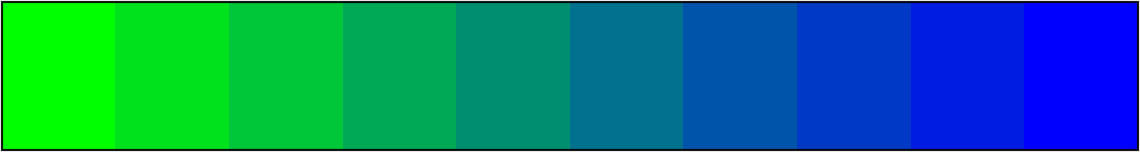
\includegraphics[width = 7cm]{\here/colorbarRGB.png}};
	\node[inner sep = 0pt, anchor = north, yshift = -0.2cm] (n2) at (n1.south)  {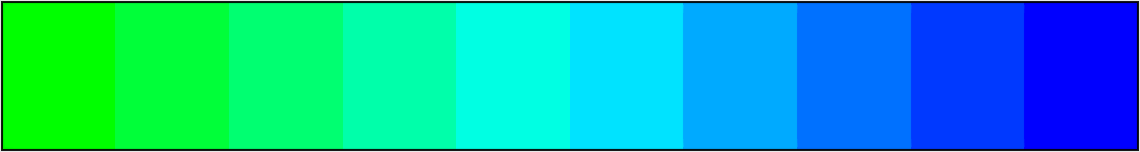
\includegraphics[width = 7cm]{\here/colorbarHSV.png}};
	\node[inner sep = 0pt, anchor = north, yshift = -0.2cm] (n3) at (n2.south) {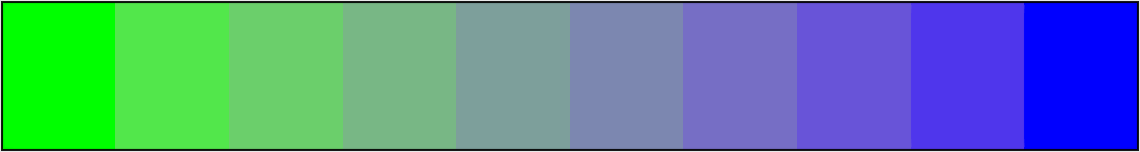
\includegraphics[width = 7cm]{\here/colorbarLab.png}};

	\node[anchor = east] at (n1.west){RGB};
	\node[anchor = east] at (n2.west){HSV};
	\node[anchor = east] at (n3.west){Lab};

\end{tikzpicture}
\end{minipage}
\end{figure} 

The key takeaway here is that a reasonable colors distance metric is not necessarily determined by an Eucledian color space distance, but by how the human eye and brain interpret those differences. A well-designed colormap is \emph{perceptually uniform}: Equal steps in the data should correspond to equal perceived changes in color---just as a fixed distance on the $x$ axis of a plot always represents the same step in scale. For example, in a topographic elevation map, a shift from 1500 meters to 1200 meters below sea level (represented by a change from dark to lighter blue) should be perceived as the same elevation increase as a shift from 1000 meters to 1300 meters above sea level (which might be represented by a transition from tan to a lighter tan).
Unsurprisingly, the human vision is a very complex issue and one that requires extensive empirical studies, see e.g. Refs.~\cite{rogowitz1996,mullen1985,crameri2020}. For example, research has shown that the human brain perceives changes in lightness far more effectively than changes in hue when interpreting data~\cite{rogowitz1996}. As a result, colormaps with a monotonically increasing lightness are generally more intuitive and easier to interpret for viewers.

\begin{figure}
	\centering
	\tikzsetnextfilename{fig_colordiffs}
	% tikz_colordiffs.tex

\begin{tikzpicture}

\begin{groupplot}[
		group style = {
			group name = dE,
			group size = 3 by 1,
			vertical sep = .25cm,
			horizontal sep = .25cm, 
			},
		width = 4.5cm,
		height = 4cm,
		enlargelimits = 0.05,
		simpleax1,
		ytick = {0,50,100},
		xticklabel = \empty,
		xmin = 0.5,
		xmax = 10.5,
		ymin = 0,
		ymax = 100,
		scale only axis,
		enlargelimits = false,
		xtick = {1.5,...,10.5},
		xmajorgrids = true, 
		ylabel = {lightness $L$},
		xlabel style = {yshift = -0.4cm},
		]

		\nextgroupplot[xlabel = {RGB}]
		\addplot+[hcqblue, ultra thick, mark = triangle*, mark options = {thin, fill = hcqblue, draw = black}]table[y index = 1]{coldiffLight.txt};
		%\coordinate (p1) at (rel axis cs:0,0);
		

		\nextgroupplot[xlabel = {HSV}, ylabel = \empty, yticklabel = \empty]
		\addplot+[hcqblue, ultra thick, mark = triangle*,mark options = {thin, fill = hcqblue, draw = black}]table[y index = 2]{coldiffLight.txt};

		\nextgroupplot[xlabel = {Lab}, ylabel = \empty, yticklabel = \empty]
		\addplot+[hcqblue, ultra thick, mark = triangle*,mark options = {thin, fill = hcqblue, draw = black}]table[y index = 3]{coldiffLight.txt};

\end{groupplot}

\node[draw = black, thick, inner sep = 0pt, anchor = north] at (dE c1r1.south){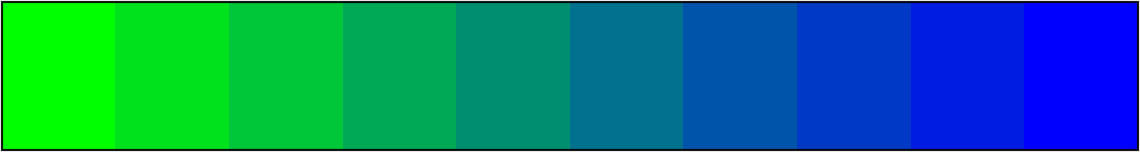
\includegraphics[width = 4.5cm]{\here/colorbarRGB.png}};
\node[draw = black, thick, inner sep = 0pt, anchor = north] at (dE c2r1.south){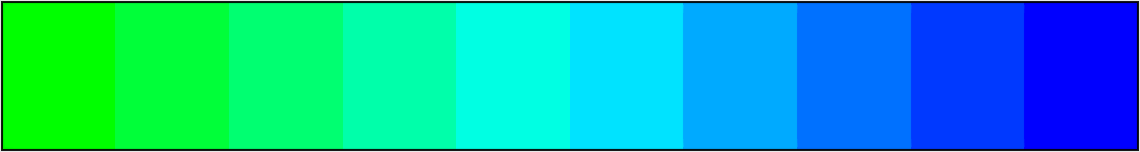
\includegraphics[width = 4.5cm]{\here/colorbarHSV.png}};
\node[draw = black, thick, inner sep = 0pt, anchor = north] at (dE c3r1.south){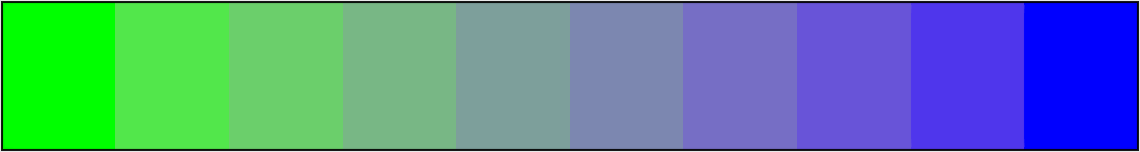
\includegraphics[width = 4.5cm]{\here/colorbarLab.png}};



\begin{groupplot}[
		group style = {
			group size = 3 by 1,
			vertical sep = .25cm,
			horizontal sep = .25cm, 
			},
		width = 4.5cm,
		height = 4cm,
		enlargelimits = 0.05,
		simpleax1,
		ytick = {0,12.5,25,37.5,50},
		xticklabel = \empty,
		yticklabels = {0,,,,50},
		xmin = 0.5,
		xmax = 10.5,
		ymin = 0,
		ymax = 50,
		ytick pos = right, 
		yticklabel pos = right,
		scale only axis,
		ylabel = {color difference},
		ylabel style = {yshift = 0.2cm},
		enlargelimits = false,
		xtick = {1.5,...,10.5},
		legend style = {
			at = {(0.5,1)},
			anchor = south,
			legend1},
		legend columns = 3
		]


		\nextgroupplot[ylabel = \empty, yticklabel = \empty]
		\addplot+[hcqyellow, ultra thick, mark options = {thin, fill = hcqyellow, draw = black}]table[y index = 1]{coldiffLab.txt};
		\addplot+[hcqred, ultra thick, mark options = {thin, fill = hcqred, draw = black}]table[y index = 1]{coldiff2000.txt};

		\addlegendentry{$\Delta E^*_{ab}$}
		\addlegendentry{$\Delta E^*_{2000}$}
		\addlegendimage{hcqblue, ultra thick, mark = triangle*, mark options = {thin, fill = hcqblue, draw = black}};
		\addlegendentry{$L$};
		

		\nextgroupplot[ylabel = \empty, yticklabel = \empty]
		\addplot+[hcqyellow, ultra thick, mark options = {thin, fill = hcqyellow, draw = black}]table[y index = 2]{coldiffLab.txt};
		\addplot+[hcqred, ultra thick, mark options = {thin, fill = hcqred, draw = black}]table[y index = 2]{coldiff2000.txt};

		\addlegendentry{$\Delta E^*_{ab}$}
		\addlegendentry{$\Delta E^*_{2000}$}
		\addlegendimage{hcqblue, ultra thick, mark = triangle*, mark options = {thin, fill = hcqblue, draw = black}};
		\addlegendentry{$L$};


		\nextgroupplot[]
		\addplot+[hcqyellow, ultra thick, mark options = {thin, fill = hcqyellow, draw = black}]table[y index = 3]{coldiffLab.txt};
		\addplot+[hcqred, ultra thick, mark options = {thin, fill = hcqred, draw = black}]table[y index = 3]{coldiff2000.txt};


		\addlegendentry{$\Delta E^*_{ab}$}
		\addlegendentry{$\Delta E^*_{2000}$}
		\addlegendimage{hcqblue, ultra thick, mark = triangle*, mark options = {thin, fill = hcqblue, draw = black}};
		\addlegendentry{$L$};

	\end{groupplot}

	\node[text width=1em, anchor=west]at(dE c1r1.north west){\subcaptionbox{\label{dEa}}{}};
	\node[text width=1em, anchor=west]at(dE c2r1.north west){\subcaptionbox{\label{dEb}}{}};
	\node[text width=1em, anchor=west]at(dE c3r1.north west){\subcaptionbox{\label{dEc}}{}};
\end{tikzpicture}

	\caption{\textbf{Lightness and color distances.} The three panels show the lightness $L$, as well as tow different color metrics for uniformely spaced in colors in (a) RGB, (b) HSV, and (c) Lab color space. For details, see the main text.}
	\label{fig:colordiffs}
\end{figure}

In \figref{fig:colordiffs}, we analyze the lightness (blue line) of the colors in the colormaps from \figref{fig:colorspaces} to see if our intuition (Lab is the best, followed by RGB, and then HSV) holds true.
The three panels confirm our anticipation:
\begin{itemize}
\item The RGB colors (left) exhibit a relatively constant change in lightness in the greenish range, but plateau near the blue end, making the last colors harder to distinguish.
\item The HSV colors (middle) maintain an almost constant lightness near the initial color, which matches our earlier judgment that the greenish hues are barely distinguishable.
\item The Lab colors (right) display a uniform decrease in lightness, ensuring well-distinguished colors throughout the entire range.
\end{itemize}

It is no coincidence that Lab performs best, as the Lab color space is designed to be perceptually uniform and maintain consistent perceptual differences when picking regularly spaced $(L,a,b)$ points. The $L$ component directly represents lightness. There are more color spaces designed to reflect human color vision, the earliest being CIEXYZ\footnote{CIE stands for Commission internationale de l'éclairage, which is french for International Commission on Illumination}, defined in 1931. It was developed using experimental data from human test subjects. However, CIEXYZ is not perceptually uniform, leading to the introduction of CIELAB (Lab) and CIELUV (Luv) in 1976, which aimed to address this limitation.

The CIE also introduced various color distance metrics, typically denoted as $\Delta E^*$, where $E$ stands for the German word `Empfindung'. The first definition, called $\Delta E^*_{ab}$, was simply the Eucledian distance in the Lab color space. As the understanding of human color perception evolved, non-uniformities in the CIELAB space, particularly in highly saturated regions, where discovered. To improve accuracy, better distance metrics were developed. The most advanced is CIEDE2000 $\Delta E^*_{00}$, which aligns with the latest research on human color vision. 
\figref{fig:colordiffs} also depicts $\Delta E^*_{ab}$ and $\Delta E^*_{00}$. 
Per definition, $\Delta E^*_{ab}$ remains constant for the Lab colors, while it peaks in the other two cases and decreases toward the edges. For $\Delta E^*_{00}$, the absolute magnitude is particularly significant: as noted earlier, colors in the green (HSV) and blue (RGB) regions are hard to distinguish. This is reflected in the $\Delta E^*_{00}$ values, which approach zero in those areas, whereas in the Lab space, a certain minimum distance is consistently maintained.


\subsection{Mach bands in diverging color maps}

Diverging colormaps typically pass through an unsaturated midpoint, often white. As a result, creating a perceptually uniform colormap by interpolating colors in the Lab color space (as done previously) is not possible. One possible approach is piecewise interpolation, i.e., moving from one color to white and then taking a sharp turn.  Such a sudden transition from increasing to decreasing lightness can activate the human eye's edge-detection mechanisms and create artificial visual features called Mach bands. It is often beneficial to soften the lightness gradient near the midpoint to avoid abrupt visual edges. This comes at the cost of a slight perceptual flat spot around the vanishing lightness gradient. For technical details on how to smoothen the lightness transition, see, e.g., Refs.~\cite{moreland2009,kovesi2015}.

\figref{fig:machbands} compares two diverging colormaps (taken from Ref.~\cite{moreland2009}) applied to the function $f(x) = \cos x + \cos y$. The colormaps share identical edge colors, but (a) has a sharp peak in lightness, while (c) has a smoother transition. The respective lightness values are shown in panel (b). In (a), the peak creates white Mach bands, whereas in (c), these artificial features are absent, thanks to the flattened lightness transition.
While (c) may be preferable in many situations, it is not always the better choice. In some cases, a sharp transition can be desirable, especially when the white midpoint carries specific significance. For example, in \figref{fig:machbands}, the contour lines where $f(x)=0$ could represent the Fermi lines of a square lattice tight-binding model. If the goal is to highlight the precise shape of the Fermi line, a sharp contrast can be advantageous.

In summary, when selecting a diverging colormap, be mindful of potential artifacts and carefully consider whether these are undesirable or beneficial.

\begin{figure}
	\centering
	\tikzsetnextfilename{fig_machbands}
	% This is the Mach band plot.
\begin{tikzpicture} 
	\begin{groupplot}[
		group style = {
			group name = name1,
			group size = 3 by 1,
			vertical sep = .25cm,
			horizontal sep = .15cm, 
			},
			view={0}{90},
			simpleax1,
			width = .7*\axisdefaultwidth,
			height = .7*\axisdefaultwidth,
			simpleax1,
			xtick = {-6.28,0,6.28},
			xticklabels = {$-2\pi$, $0$, $2\pi$},
			ytick = {-6.28,0,6.28},
			yticklabels = {$-2\pi$, $0$, $2\pi$},
			xlabel = $x$,
			ylabel = $y$,
			scatter/use mapped color={
       			draw=black,
        		fill=mapped color,
    		}, 
			ylabel style = {yshift = -0.4cm},
			colorbar horizontal,
			colorbar style={
					axis line style = {line cap=rect},
					ticklabel style = {font=\footnotesize},
					thick,
					at={(0,1.02)},            
					anchor=below south west, 
					width=1*\pgfkeysvalueof{/pgfplots/parent axis width},
					xticklabel pos=upper,
					xlabel = {$f(x)$},
					axis on top,
					xtick pos=right,
					xlabel near ticks
				}, 
		]
	
		\nextgroupplot[colormap name = coolwarmB, colorbar] 
		\addplot3[surfstyle, domain=-6.29:6.29]{cos(deg(y)) + cos(deg(x))}; 

		\nextgroupplot[xmin=0, xmax=100, xshift = .6cm, ylabel = {lightness $L$}, xlabel = color, xtick = \empty, ymin = 37, ymax = 100, ytick = {40, 100}, yticklabels = {40, 100}, colorbar = false, ylabel style = {yshift = -0.3cm},]
		\addplot[colormap name = coolwarm, scatter, scatter src = x, ultra thin] table[]{machbands2.txt};
		\addplot[colormap name = coolwarmB, scatter, scatter src = x, ultra thin] table[y index = 2]{machbands2.txt};
		\coordinate (m1) at (axis cs: 50.0, 94.662);
		\coordinate (m2) at (axis cs: 75.0, 72.33121);

		\nextgroupplot[colormap name = coolwarm, ytick pos = right, yticklabel pos = right, ylabel style = {yshift = 0.8cm}]
		\addplot3[surfstyle, domain=-6.29:6.29]{cos(deg(y)) + cos(deg(x))}; 

	\end{groupplot} 

	\draw[-stealth, ultra thick, hcqblue] (m1) -- (m1 -| name1 c1r1.east);
	\draw[-stealth, ultra thick, hcqblue] (m2) -- (m2 -| name1 c3r1.west);

	\node[yshift = 0.3cm, text width = 1em, anchor = south east]at (name1 c1r1.north west) {\subcaptionbox{\label{mach-a}}{}};
	\node[yshift = 0.3cm, text width = 1em, anchor = south east]at (name1 c2r1.north west) {\subcaptionbox{\label{mach-b}}{}};
	\node[yshift = 0.3cm, text width = 1em, anchor = south east]at (name1 c3r1.north west) {\subcaptionbox{\label{mach-c}}{}};


\end{tikzpicture}

	\caption{\textbf{Mach bands in diverging colormaps.} Shown is the function $f(x) = \cos x + \cos y$, color-coded with a colormap with (a) a sharp change in lightness at the white point, resulting in white Mach bands and (c) a smoothened lightness evolution. Panel (b) shows the lightness values $L$ for the two colormaps.}
	\label{fig:machbands}
\end{figure}


\section{An example: Rainbow vs. good colormaps}\label{sec:rainbow}

To conclude this chapter, let's examine an example that highlights the advantages of a scientifically derived colormap and the serious drawbacks of a poorly chosen one. We consider a two-dimensional plot of the function $f(x)= \left(1 - \sqrt{y} \right)  \cos x^3$, which represents a harmonic oscillation in $x$ direction that is damped along the $y$ axis, where we restrict $y$ to $\left[0,1\right]$. This function is a rough approximation of the spatial contrast sensitivity function often used for similar purposes, as seen, e.g., in Ref.~\cite{moreland2009}. While I am unsure if a standardized definition exists, I believe my choice effectively conveys the intended message.
\figref{fig:sensitivityfunction} presents a two-dimensional plot of this function using the perceptually uniform \verb|viridis| colormap.
Notably, the oscillations remain well-resolved in the strongly damped upper region where $y \lesssim 1$.

\begin{figure}
\captionsetup{format = sidebyside, indention = 0cm} 
\begin{minipage}[t]{0.4\textwidth}
	\vspace{-5pt}
	\caption{\textbf{Spatial contrast sensitivity function},  $f(x)= \left(1 - \sqrt{y} \right)  \cos x^3$. The oscillations along the $x$ axis and the damping along the $y$ axis are clearly visible throughout the selected region of the two-dimensional $xy$ plane. In this section, we will use the resolution of these features in $f(x,y)$ to evaluate the performance of different colormaps.}
	\label{fig:sensitivityfunction}
\end{minipage}\hfill 
\begin{minipage}[t]{0.55\textwidth}
	\centering 
	\vspace{0pt}
	\tikzsetnextfilename{fig_sensitivityfunction}
	% tikz_sensitivityfunction.tex


\begin{tikzpicture}
	\begin{axis}[
			view={0}{90},
			simpleax1,
			xtick = {1,2,3},
			ytick = {0,0.5,1},
			xlabel = $x$,
			ylabel = $y$,
			colorbar horizontal,
			colorbar style={
					axis line style = {line cap=rect},
					ticklabel style = {font=\footnotesize},
					thick,
					at={(0,1.02)},   
					% xtick = {-1.5,0,1.5},       
					anchor=below south west, 
					width=1*\pgfkeysvalueof{/pgfplots/parent axis width},
					xticklabel pos=upper,
					xlabel = {$f(x)$},
					axis on top,
					xtick pos=right,
					xlabel near ticks,
				}, 
			colormap name = viridis
		]
	
		\addplot3[samples = 100, surfstyle, domain=0.7:3, y domain = 0:1]{(1 - y ^(1/2)) * cos(deg(x^3))}; 
	
	\end{axis}
\end{tikzpicture}
\end{minipage}
\end{figure} 


Next, we will consider the same plot using three different colormaps and their colorblind and monochromatic versions.
Specifically, we will consider
\begin{itemize}
\item the \verb|cividis| colormap, introduced in Ref.~\cite{nunez2018}. This colormap is derived from the \verb|viridis| scheme and modified to optimize readability for colorblind readers as the cost of being less aesthetically pleasing (in the opinion of the creators of that colormap \cite{nunez2018}).
\item the \verb|batlow| colormap, one of several perceptually uniform colormaps designed by Fabio Crameri and introduced in Ref.~\cite{crameri2020}
\item the \verb|gist_rainbow| colormap as an example for a really bad colormap that obscures data, introduce artificial features, and, therefore confuses users.
\end{itemize}

In fact, rainbow color maps are more widespread than one might expect given their well-documented shortcomings. 
It wasn't too long ago that rainbow maps were the standard color schemes of many common plotting libraries, e.g., the \verb|jet| colormap in Matplotlib before the 2.0 release in 2017.
In the 2000's, rainbow-like colormaps were by far the most common colormaps in scientific visualization CITE.
In recent years, the awareness about the problems has increased, witnessed by the advent of many good alternatives, \verb|viridis| being the most popular.

One can already gain insights from the colorbars of the corresponding maps. Those are shown in \figref{fig:colorbars}. In addition to the original colors, the most common types of color blindness are also considered, along with the colorbar after grayscale conversion. Note that in contrast to \figref{fig:lineplotcolorblindness}, we assume total instead of only partial loss of one of the three types of human photopigments (i.e., deuteranopia, not deuteranomaly, etc.) 

The main observations are: (i) The \verb|cividis| and \verb|batlow| colormaps exhibit a clear and uniform progression toward higher brightness, which is consistently maintained across all color blindness variants. (ii) \verb|cividis| does not include green or red tones, so the colors in protanopia or deuteranopia hardly change at all. (iii) The \verb|gist_rainbow| colormap shows distinct brightness peaks in yellow and cyan, with intermediate areas where the color appears almost unchanged, particularly in the green range. These extended flat regions are especially problematic for colorblind readers. For instance, with protanopia, there are essentially only four broad areas of nearly constant color (gray, yellow, white, and blue), with very short transitions between them. Additionally, the colors lack a clear order, which is most apparent in the monochrome version: multiple recurring light and dark regions make it impossible to determine which color represents high or low numerical values.
It is easy to imagine that this colormap leaves ample space for misinterpretation of data, even for non-colorblind readers. Let us now look at the spatial contrast sensitivity function to see whether this expectation is confirmed.





\begin{figure}
	\centering
	\tikzsetnextfilename{fig_colorbars}
	% tikz_colorbars.tex

\begin{tikzpicture} 
	
	\node[inner sep = 0pt] (c1) {
\includegraphics[width = 4.1cm]{\here/colorbars/cividis.png}};
	\node[inner sep = 0pt, anchor = north, yshift = -0.1cm] (c2) at (c1.south)  {
\includegraphics[width = 4.1cm]{\here/colorbars/cividis_prot.png}};
	\node[inner sep = 0pt, anchor = north, yshift = -0.1cm] (c3) at (c2.south) {
\includegraphics[width = 4.1cm]{\here/colorbars/cividis_deut.png}};
	\node[inner sep = 0pt, anchor = north, yshift = -0.1cm] (c4) at (c3.south) {
\includegraphics[width = 4.1cm]{\here/colorbars/cividis_trit.png}};
	\node[inner sep = 0pt, anchor = north, yshift = -0.1cm] (c5) at (c4.south) {
\includegraphics[width = 4.1cm]{\here/colorbars/cividis_mono.png}};


	\node[anchor = west, xshift = 0.1cm, inner sep = 0pt] (b1) at (c1.east) {
\includegraphics[width = 4.1cm]{\here/colorbars/batlow.png}};
	\node[inner sep = 0pt, anchor = north, yshift = -0.1cm] (b2) at (b1.south)  {
\includegraphics[width = 4.1cm]{\here/colorbars/batlow_prot.png}};
	\node[inner sep = 0pt, anchor = north, yshift = -0.1cm] (b3) at (b2.south) {
\includegraphics[width = 4.1cm]{\here/colorbars/batlow_deut.png}};
	\node[inner sep = 0pt, anchor = north, yshift = -0.1cm] (b4) at (b3.south) {
\includegraphics[width = 4.1cm]{\here/colorbars/batlow_trit.png}};
	\node[inner sep = 0pt, anchor = north, yshift = -0.1cm] (b5) at (b4.south) {
\includegraphics[width = 4.1cm]{\here/colorbars/batlow_mono.png}};


	\node[anchor = west, xshift = 0.1cm, inner sep = 0pt] (r1) at (b1.east) {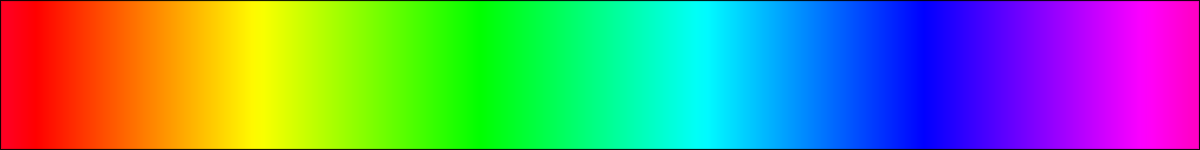
\includegraphics[width = 4.1cm]{\here/colorbars/rb.png}};
	\node[inner sep = 0pt, anchor = north, yshift = -0.1cm] (r2) at (r1.south)  {
\includegraphics[width = 4.1cm]{\here/colorbars/rb_prot.png}};
	\node[inner sep = 0pt, anchor = north, yshift = -0.1cm] (r3) at (r2.south) {
\includegraphics[width = 4.1cm]{\here/colorbars/rb_deut.png}};
	\node[inner sep = 0pt, anchor = north, yshift = -0.1cm] (r4) at (r3.south) {
\includegraphics[width = 4.1cm]{\here/colorbars/rb_trit.png}};
	\node[inner sep = 0pt, anchor = north, yshift = -0.1cm] (r5) at (r4.south) {
\includegraphics[width = 4.1cm]{\here/colorbars/rb_mono.png}};

	\node[anchor = east, font = \footnotesize] at (c1.west){original};
	\node[anchor = east, font = \footnotesize] at (c2.west){protanopia};
	\node[anchor = east, font = \footnotesize] at (c3.west){deuteranopia};
	\node[anchor = east, font = \footnotesize] at (c4.west){tritanopia};
	\node[anchor = east, font = \footnotesize] at (c5.west){monochrome};

	\node[anchor = south, font = \footnotesize] at (c1.north){\texttt{cividis}};
	\node[anchor = south, font = \footnotesize] at (b1.north){\texttt{batlow}};
	\node[anchor = south, font = \footnotesize] at (r1.north){\texttt{gist\_rainbow}};

\end{tikzpicture}
	\caption{xxx}
	\label{fig:colorbars}
\end{figure}


\subsection{The original colormap}
\subsection{Color vision deficiency}





% \begin{figure}
% 	\centering
% 	\tikzsetnextfilename{fig_sensitivityCVD}
% 	% tikz_sensitivityCVD.tex

\begin{tikzpicture} 
	
	\node[draw = black, thick, inner sep = 0pt] (c11) {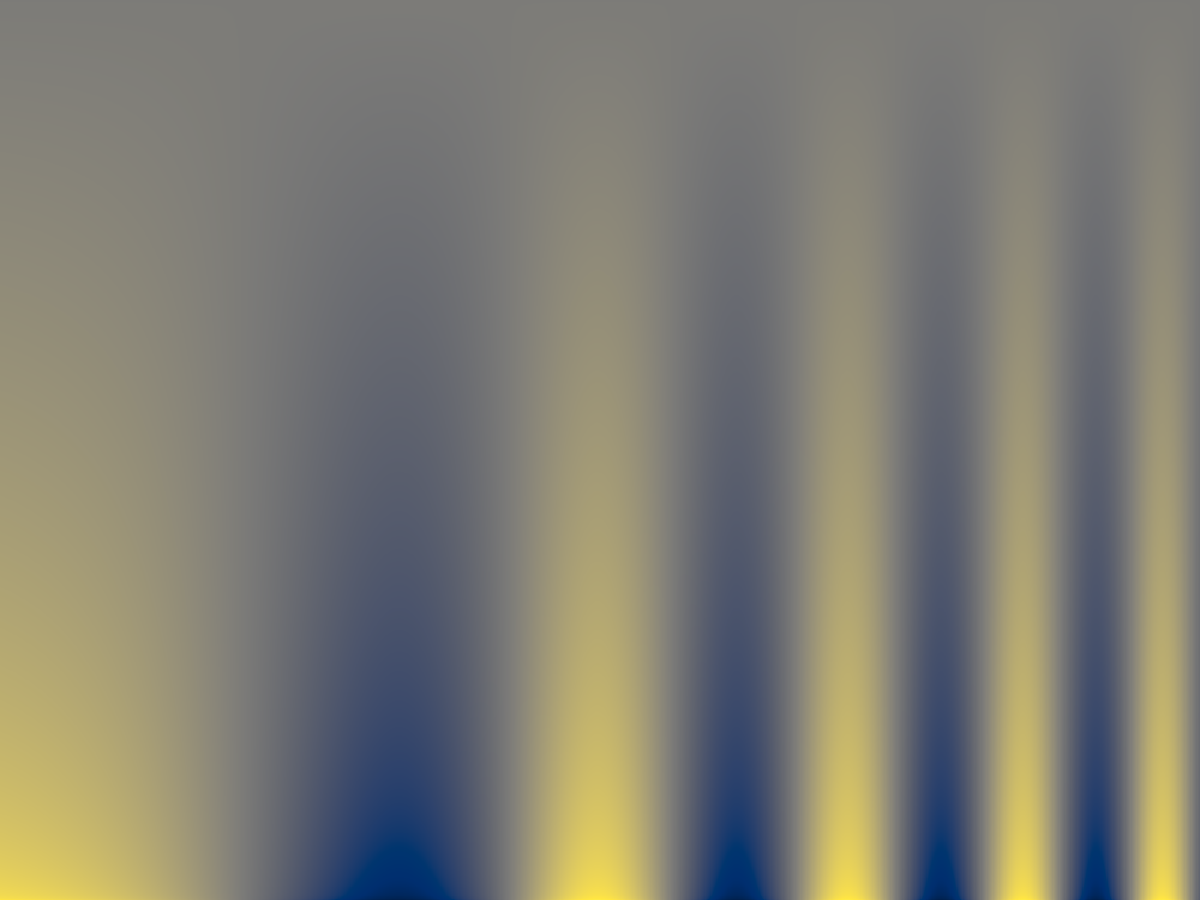
\includegraphics[width = 4.5cm]{\here/sensitivity/sensitivity_11.png}};
	\node[draw = black, thick, inner sep = 0pt, anchor = north, yshift = -0.2cm] (c21) at (c11.south)  {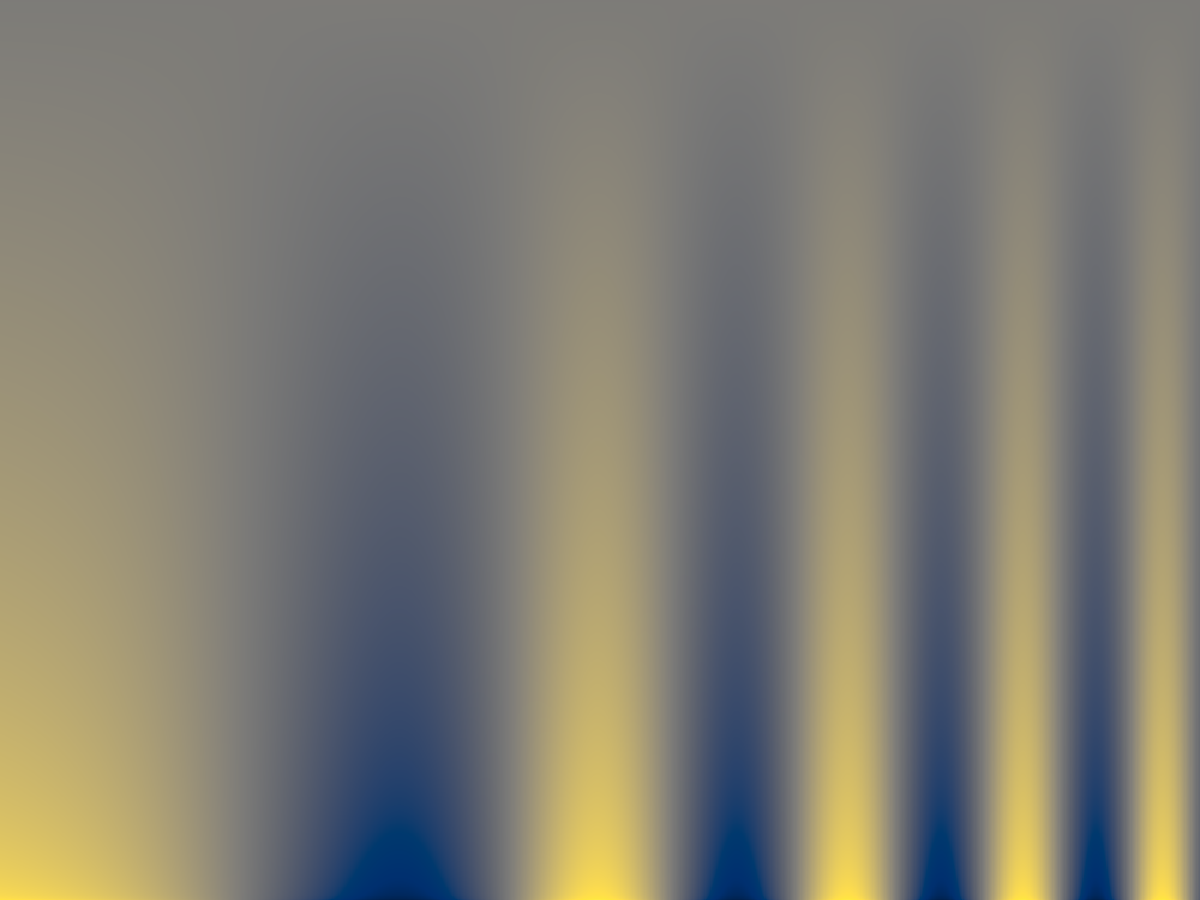
\includegraphics[width = 4.5cm]{\here/sensitivity/sensitivity_21.png}};
	\node[draw = black, thick, inner sep = 0pt, anchor = north, yshift = -0.2cm] (c31) at (c21.south) {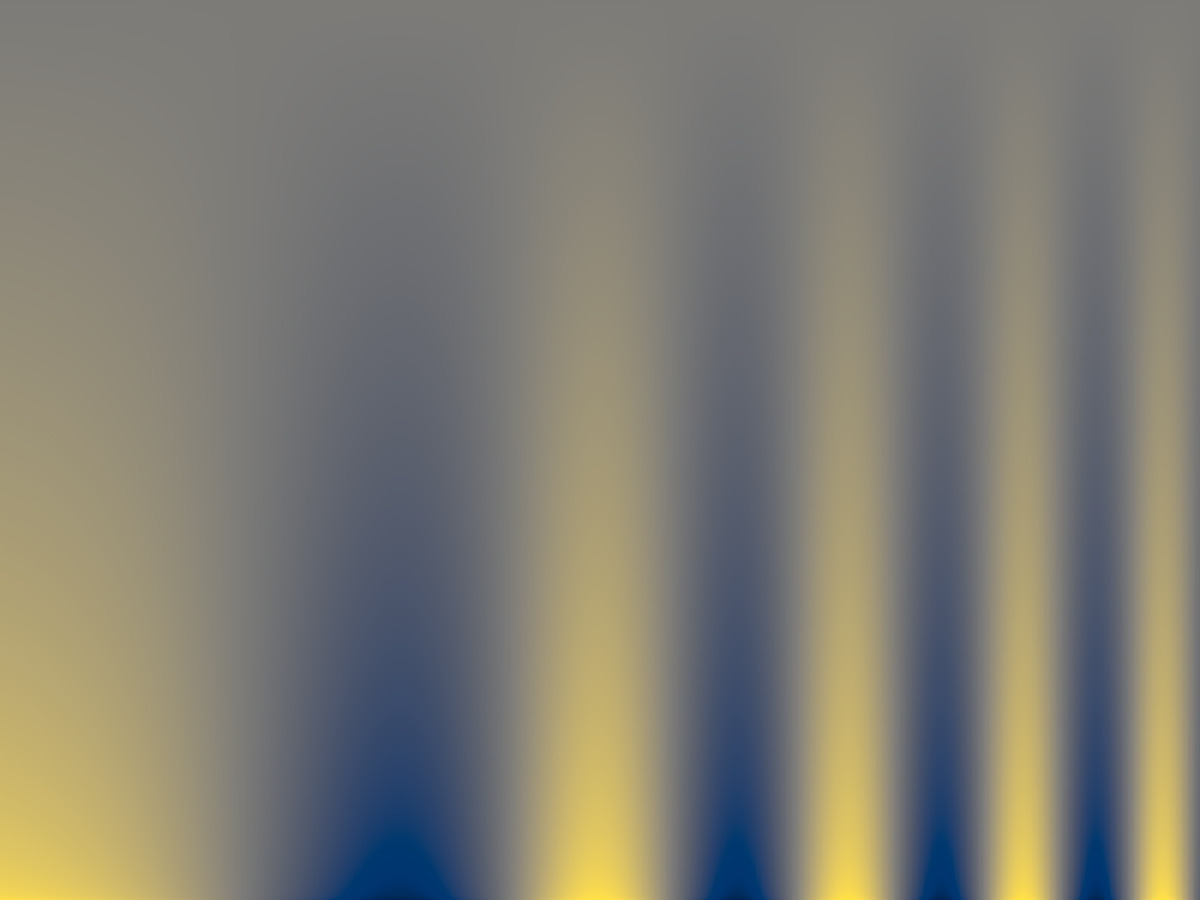
\includegraphics[width = 4.5cm]{\here/sensitivity/sensitivity_31.png}};
	\node[draw = black, thick, inner sep = 0pt, anchor = north, yshift = -0.2cm] (c41) at (c31.south) {
\includegraphics[width = 4.5cm]{\here/sensitivity/sensitivity_41.png}};
	\node[draw = black, thick, inner sep = 0pt, anchor = north, yshift = -0.2cm] (c51) at (c41.south) {
\includegraphics[width = 4.5cm]{\here/sensitivity/sensitivity_51.png}};

	\node[draw = black, thick, inner sep = 0pt, anchor = west, xshift = 0.3cm] (b12) at (c11.east){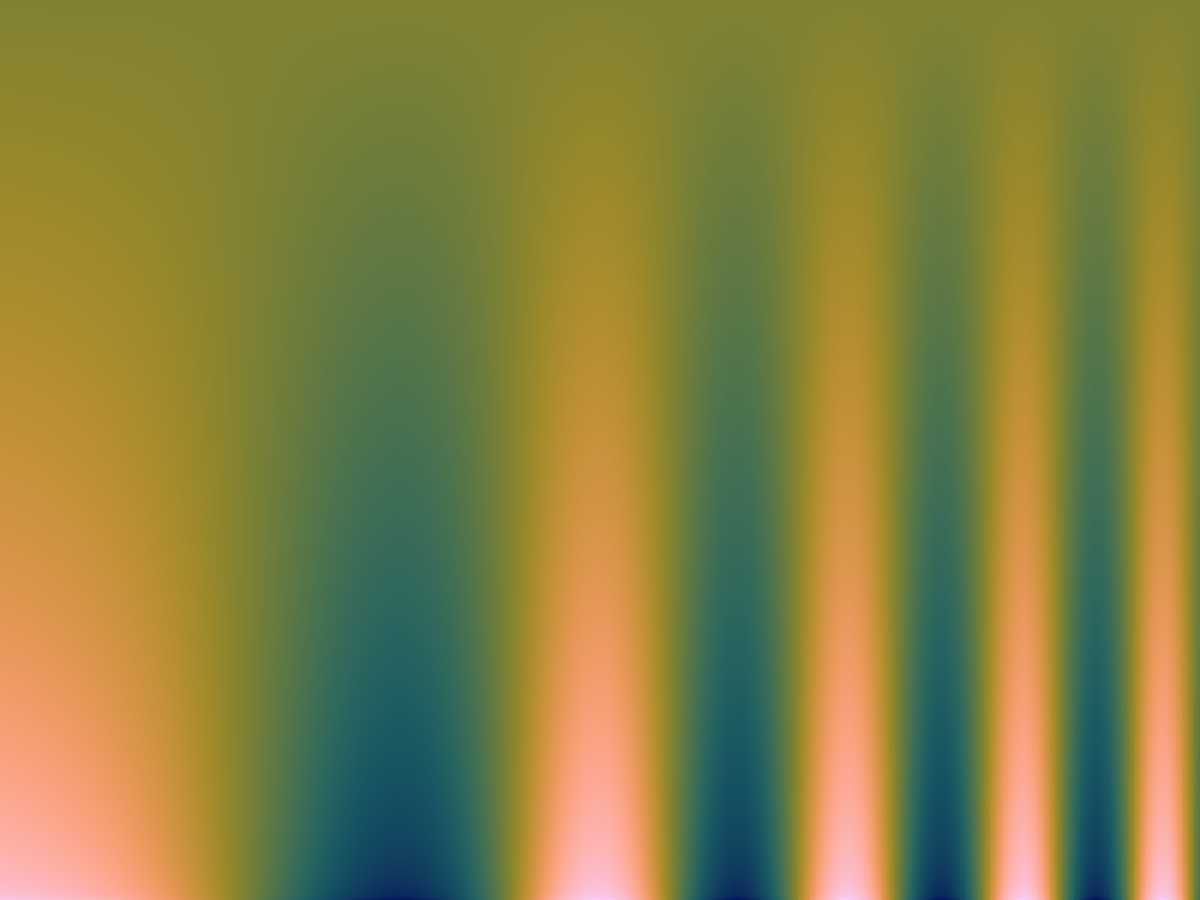
\includegraphics[width = 4.5cm]{\here/sensitivity/sensitivity_12.png}};
	\node[draw = black, thick, inner sep = 0pt, anchor = north, yshift = -0.2cm] (b22) at (b12.south)  {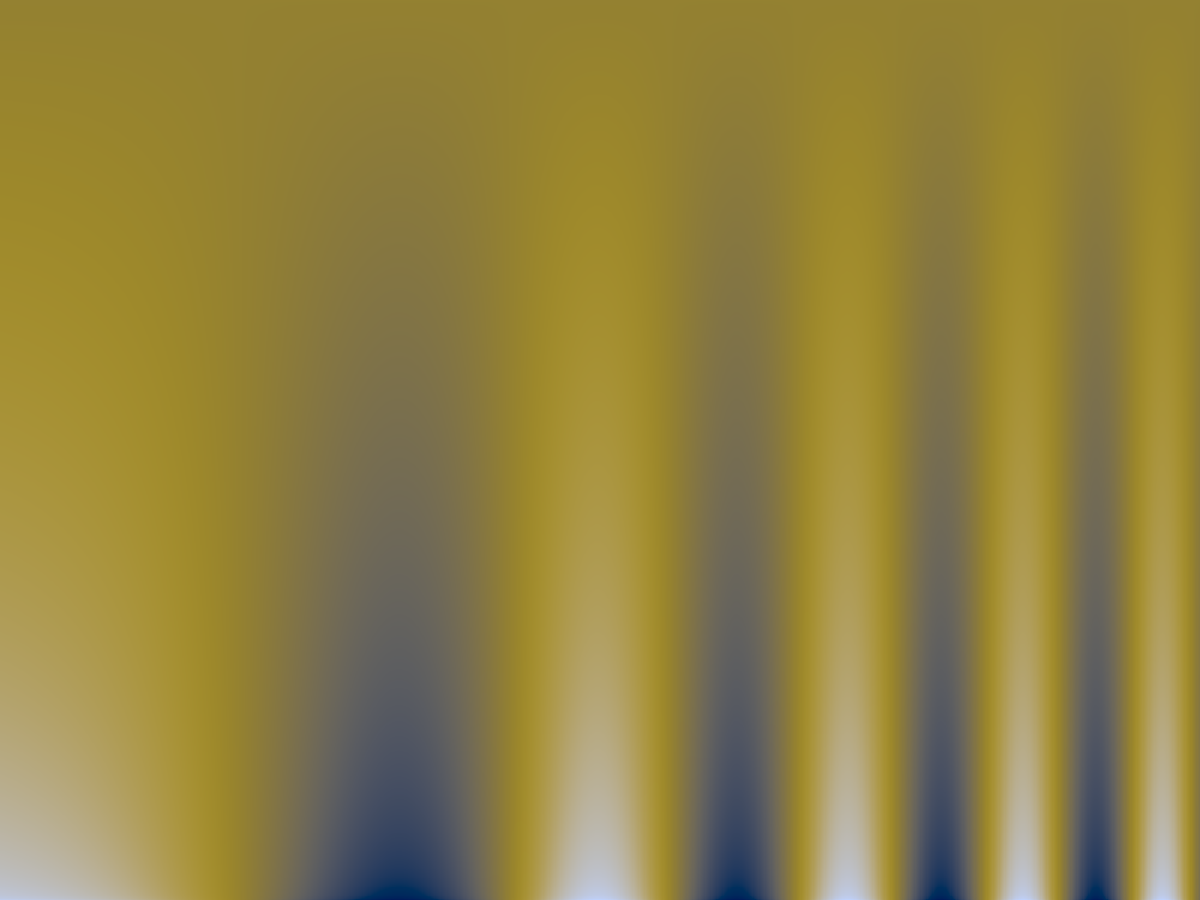
\includegraphics[width = 4.5cm]{\here/sensitivity/sensitivity_22.png}};
	\node[draw = black, thick, inner sep = 0pt, anchor = north, yshift = -0.2cm] (b32) at (b22.south) {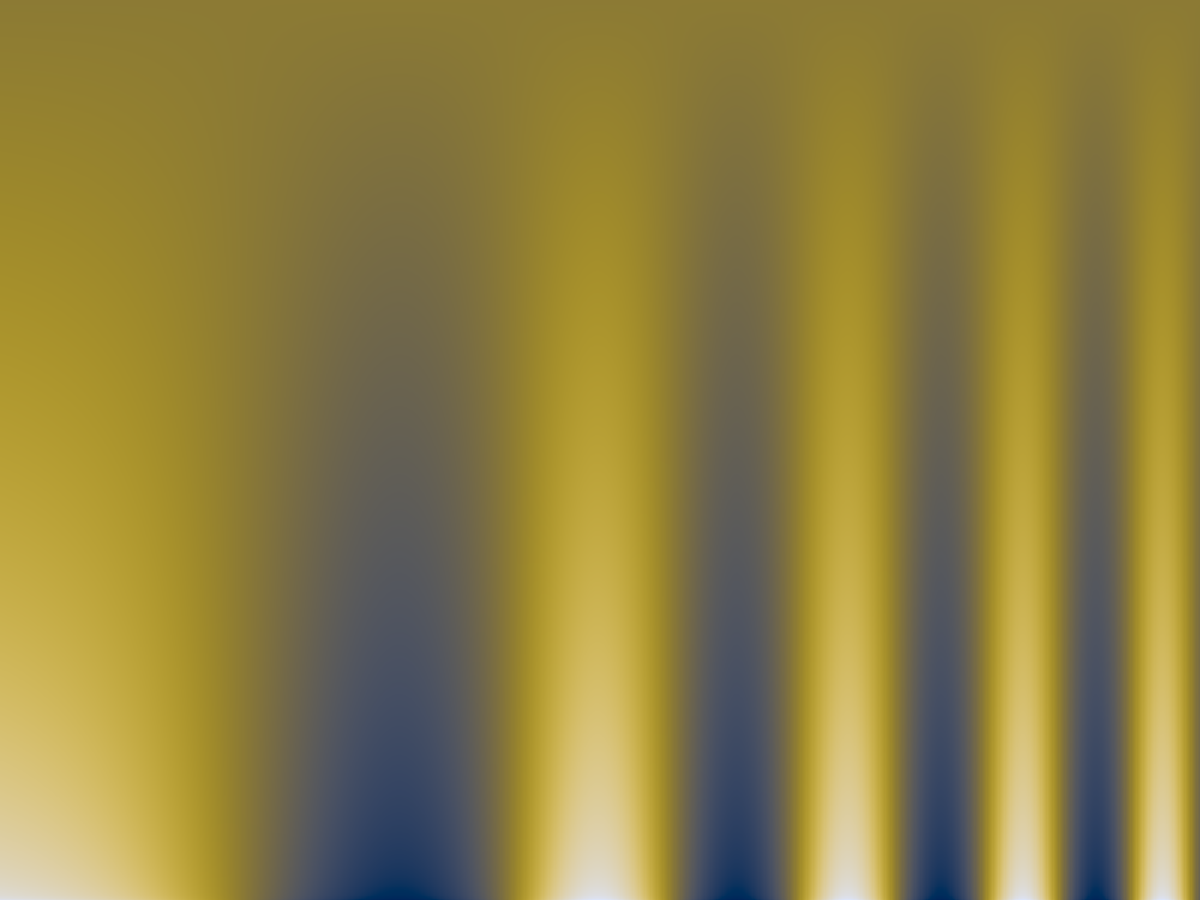
\includegraphics[width = 4.5cm]{\here/sensitivity/sensitivity_32.png}};
	\node[draw = black, thick, inner sep = 0pt, anchor = north, yshift = -0.2cm] (b42) at (b32.south) {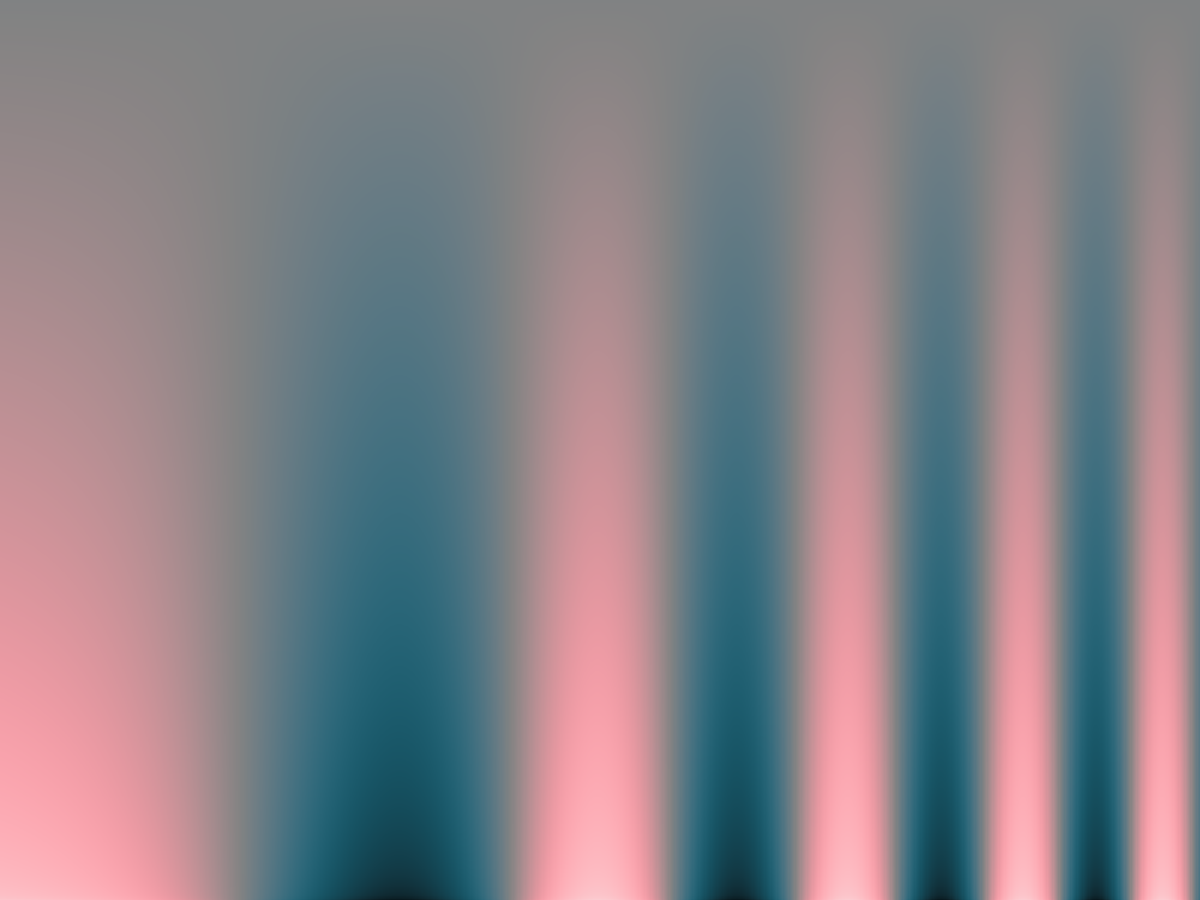
\includegraphics[width = 4.5cm]{\here/sensitivity/sensitivity_42.png}};
	\node[draw = black, thick, inner sep = 0pt, anchor = north, yshift = -0.2cm] (b52) at (b42.south) {
\includegraphics[width = 4.5cm]{\here/sensitivity/sensitivity_52.png}};


	\node[draw = black, thick, inner sep = 0pt, anchor = west, xshift = 0.3cm] (r12) at (b12.east){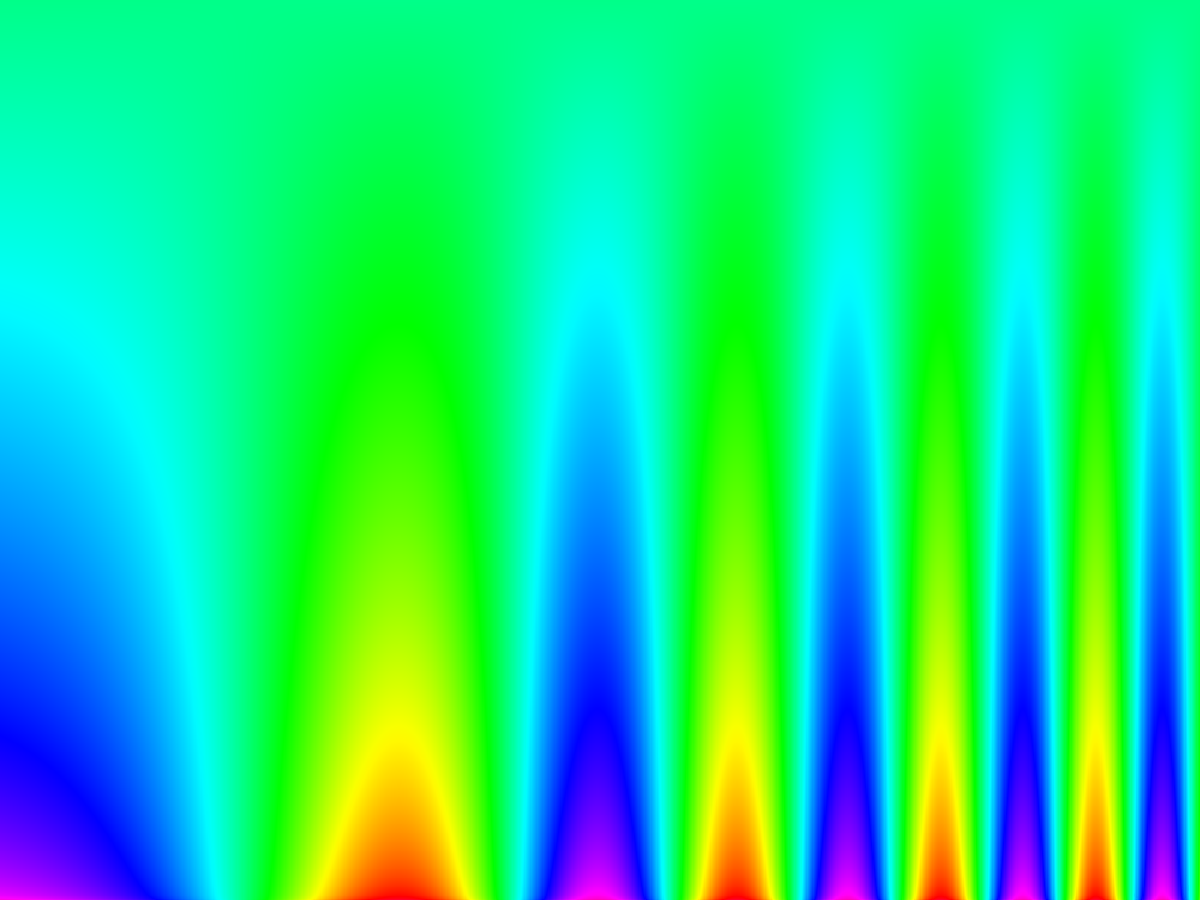
\includegraphics[width = 4.5cm]{\here/sensitivity/sensitivity_13.png}};
	\node[draw = black, thick, inner sep = 0pt, anchor = north, yshift = -0.2cm] (r22) at (r12.south)  {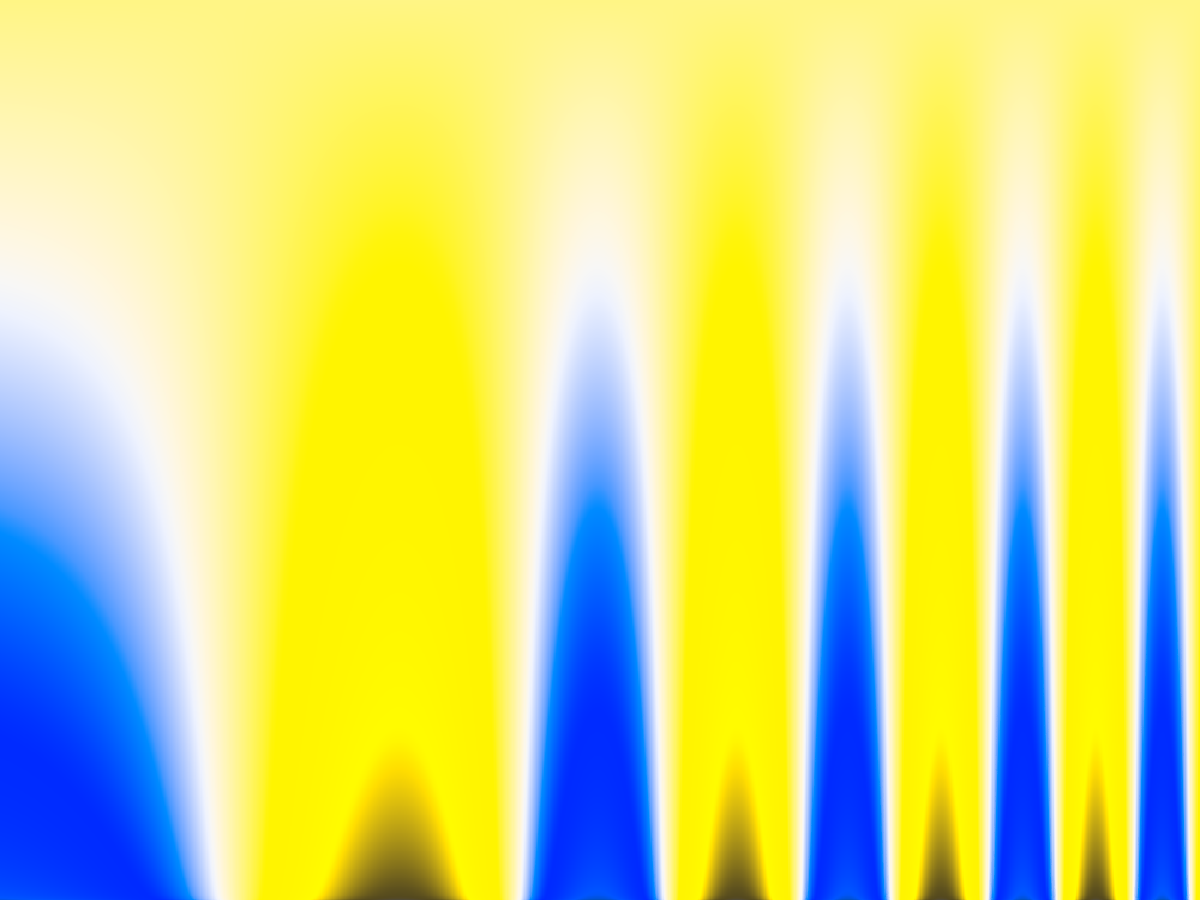
\includegraphics[width = 4.5cm]{\here/sensitivity/sensitivity_23.png}};
	\node[draw = black, thick, inner sep = 0pt, anchor = north, yshift = -0.2cm] (r32) at (r22.south) {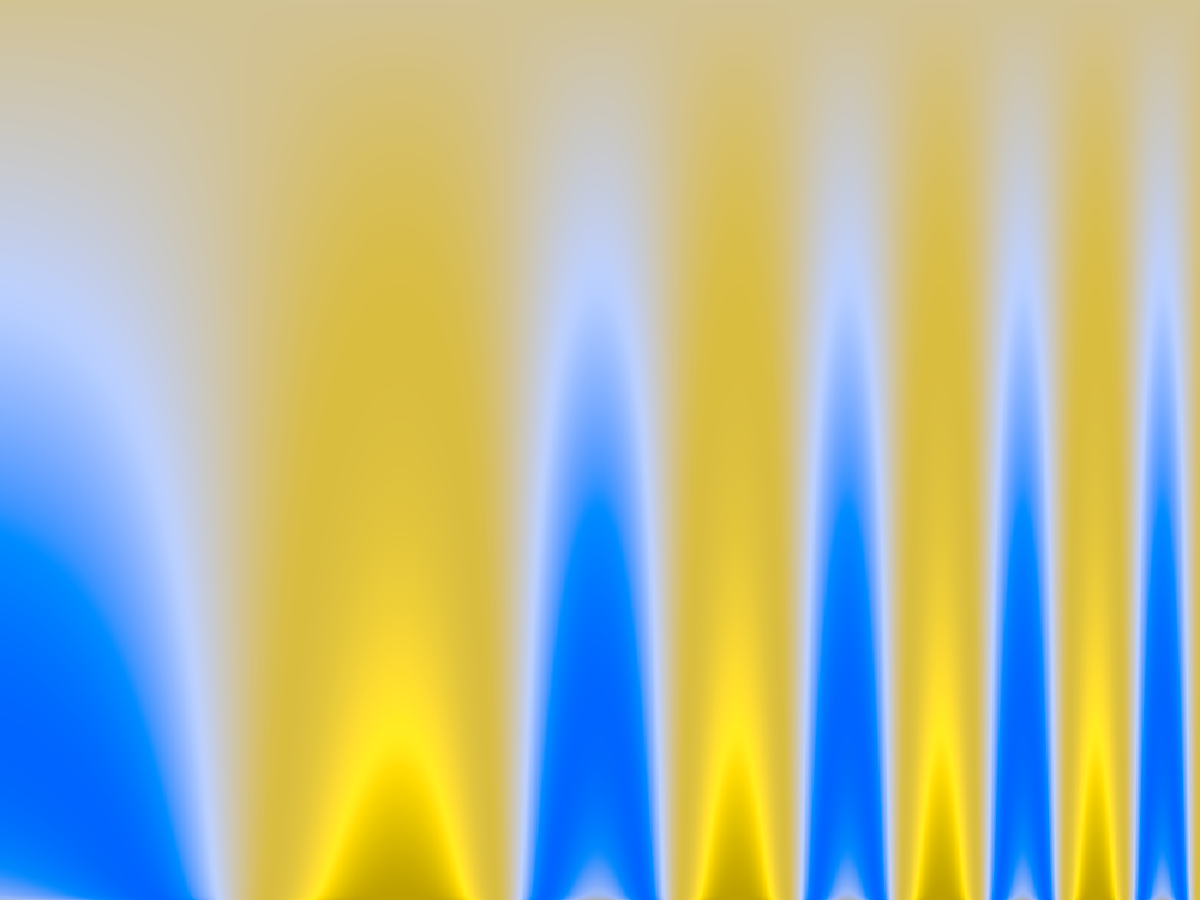
\includegraphics[width = 4.5cm]{\here/sensitivity/sensitivity_33.png}};
	\node[draw = black, thick, inner sep = 0pt, anchor = north, yshift = -0.2cm] (r42) at (r32.south) {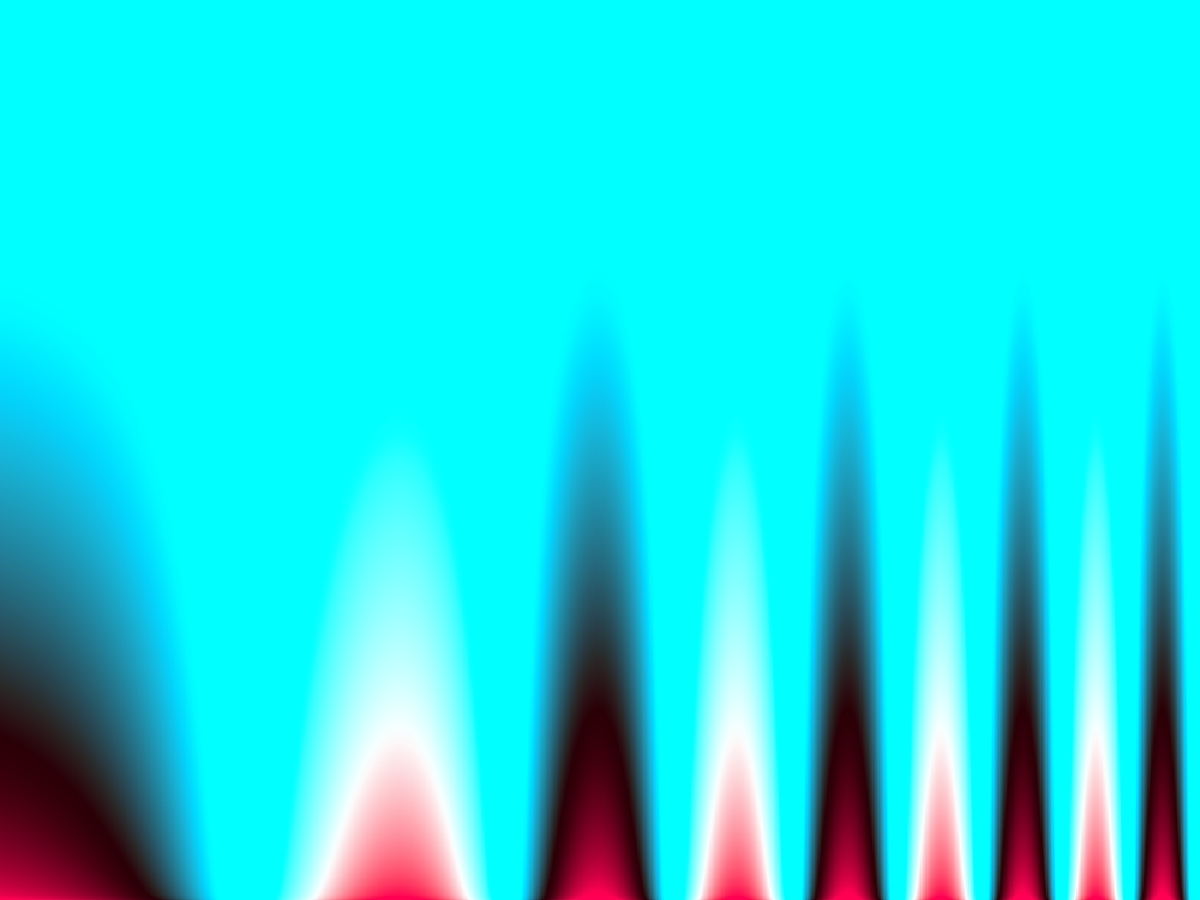
\includegraphics[width = 4.5cm]{\here/sensitivity/sensitivity_43.png}};
	\node[draw = black, thick, inner sep = 0pt, anchor = north, yshift = -0.2cm] (r52) at (r42.south) {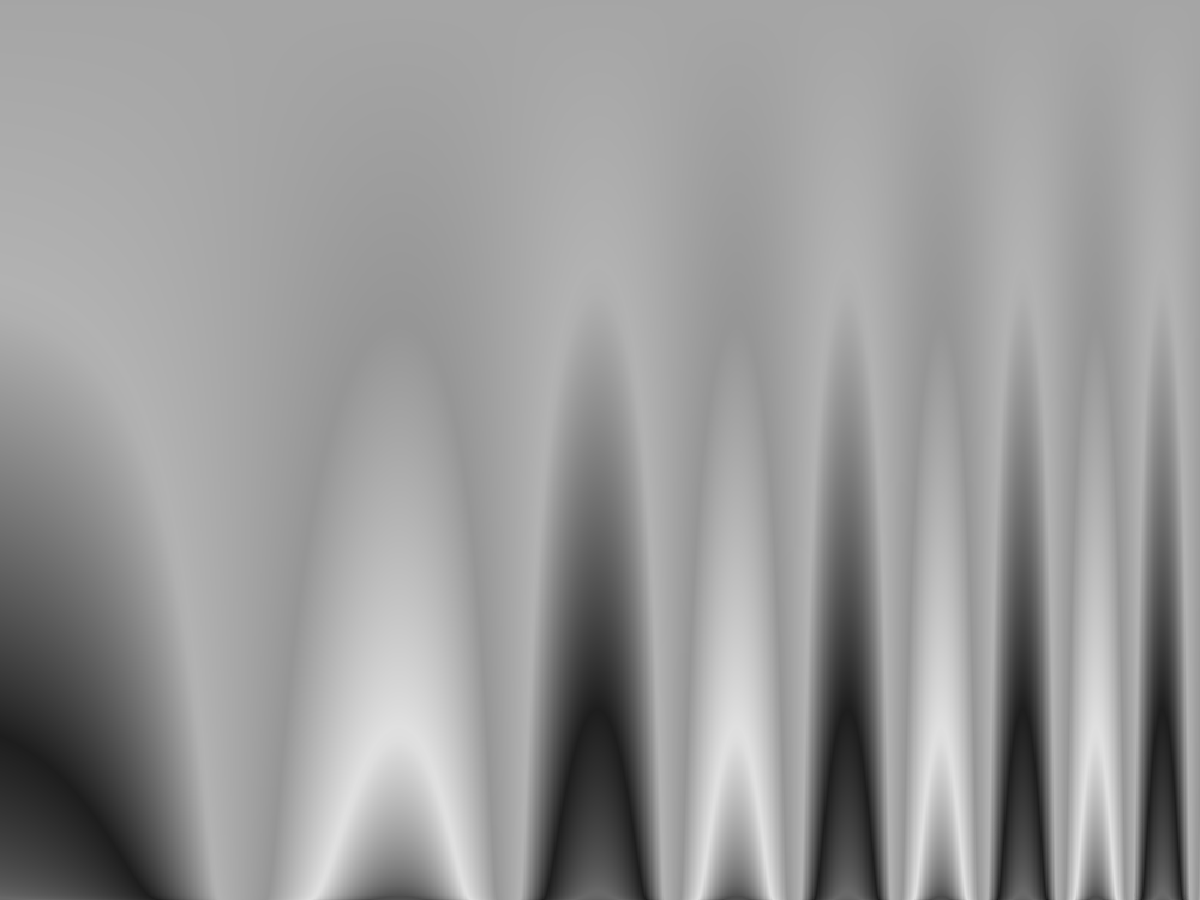
\includegraphics[width = 4.5cm]{\here/sensitivity/sensitivity_53.png}};


	\node[font = \footnotesize, anchor = east] at (c11.west){\rotatebox{90}{original}};
	\node[font = \footnotesize, anchor = east] at (c21.west){\rotatebox{90}{protanopia}};
	\node[font = \footnotesize, anchor = east] at (c31.west){\rotatebox{90}{deuteranopia}};
	\node[font = \footnotesize, anchor = east] at (c41.west){\rotatebox{90}{tritanopia}};
	\node[font = \footnotesize, anchor = east] at (c51.west){\rotatebox{90}{monochrome}};

	\node[anchor = south] at (c11.north){\texttt{cividis}};
	\node[anchor = south] at (b12.north){\texttt{batlow}};
	\node[anchor = south] at (r12.north){\texttt{gist\_rainbow}};

\end{tikzpicture}
% 	\caption{xxx}
% 	\label{fig:sensitivityCVD}
% \end{figure}

% \begin{figure}
% 	\centering
% 	\tikzsetnextfilename{fig_cmapanalytics}
% 	% tikz_cmapanalytics.tex
\pgfplotsset{
	simpleax1/.style = {
		every x tick/.style={black},
		every y tick/.style={black},
		xtick pos=left,
		ytick pos=left,
		axis on top,
		axis line style={thick, line cap = rect},
		ticklabel style = {font=\footnotesize}
	},
	surfstyle/.style = {
		surf, 
		shader=interp,
        samples=100,
	},
	colormap/RdBu,
	legend1/.style = 
	{
		font = \footnotesize,
		legend cell align={left},
		draw = none,
		/pgfplots/legend image code/.code={
			\draw[mark repeat=2,mark phase=2] 
			plot coordinates {
				(0cm,0cm) 
				(0.2cm,0cm)
				(0.4cm,0cm)
			};
		}
	},
}


\begin{tikzpicture}

\begin{groupplot}[
		group style = {
			group name = group1,
			group size = 3 by 1,
			vertical sep = .25cm,
			horizontal sep = .1cm, 
			},
		width = 4.25cm,
		height = 4cm,
		enlargelimits = 0.05,
		simpleax1,
		xticklabel = \empty,
		ymin = 0,
		ymax = 5.5,
		scatter/use mapped color={
       		draw=black,
        	fill=mapped color,
    	}, 
		scale only axis,
		enlargelimits = false, 
		ylabel = {$L$},
		ylabel style = {yshift = -0.5cm},
		legend style = {
			at = {(0.5,1)},
			anchor = south,
			legend1},
		legend columns = 3
		]

		\nextgroupplot[ytick = {0,100}, ymax = 100, ylabel = {lightness $L$}]
		\addplot[hcqblue, ultra thick]table[]{cmap_analytics/cv_L.txt};
		% \addplot[colormap/viridis, scatter, scatter src = x, ultra thin]table[]{cmap_analytics/cv_L.txt};
		\addplot[hcqyellow, ultra thick]table[]{cmap_analytics/bt_L.txt};



		\nextgroupplot[ylabel style = {yshift = 0.4cm}, ylabel = $\Delta E^*_{00}$, xshift = .9cm]
		\addplot[hcqblue, ultra thick]table[y expr =  4 *\thisrowno{1}]{cmap_analytics/cv_d.txt};
		\addplot[hcqyellow, ultra thick]table[y expr =  4*\thisrowno{1}]{cmap_analytics/bt_d.txt};

		\addlegendentry{\texttt{cividis}}
		\addlegendentry{\texttt{batlow}}
		\addlegendimage{hcqred, ultra thick};
		\addlegendentry{\texttt{gist\_rainbow}};


		\nextgroupplot[ymax = 100, ylabel = {$\Delta E_{00}^{\text{cum}}$}, ytick pos = right, yticklabel pos = right, ytick = {0,100}, ylabel style = {yshift = 0.8cm}]
		\addplot[hcqblue, ultra thick]table[]{cmap_analytics/cv_d_cum.txt};
		\addplot[hcqyellow, ultra thick]table[]{cmap_analytics/bt_d_cum.txt};


\end{groupplot}

\node[draw = black, thick, inner sep = 0pt, anchor = north] (cb1) at (group1 c1r1.south){
\includegraphics[width = 4.25cm, height = .3cm]{\here/colorbars/cividis.png}};
\node[draw = black, thick, inner sep = 0pt, anchor = north] (cb2) at (cb1.south){
\includegraphics[width = 4.25cm, height = .3cm]{\here/colorbars/batlow.png}};
\node[draw = black, thick, inner sep = 0pt, anchor = north] (cb3) at (cb2.south){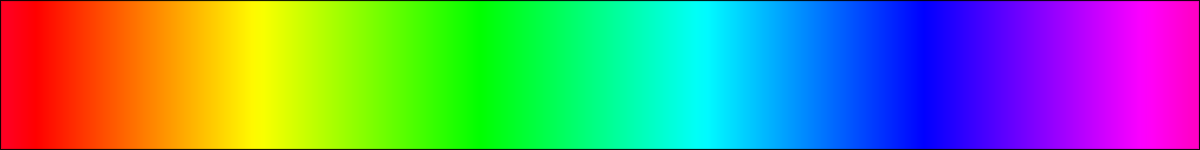
\includegraphics[width = 4.25cm, height = .3cm]{\here/colorbars/rb.png}};


\node[draw = black, thick, inner sep = 0pt, anchor = north] (cb4) at (group1 c2r1.south){
\includegraphics[width = 4.25cm, height = .3cm]{\here/colorbars/cividis.png}};
\node[draw = black, thick, inner sep = 0pt, anchor = north] (cb5) at (cb4.south){
\includegraphics[width = 4.25cm, height = .3cm]{\here/colorbars/batlow.png}};
\node[draw = black, thick, inner sep = 0pt, anchor = north] (cb6) at (cb5.south){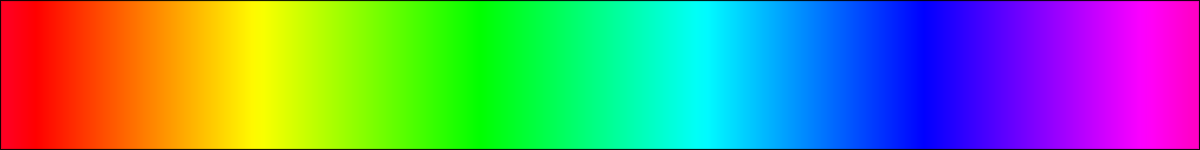
\includegraphics[width = 4.25cm, height = .3cm]{\here/colorbars/rb.png}};


\node[draw = black, thick, inner sep = 0pt, anchor = north] (cb7) at (group1 c3r1.south){
\includegraphics[width = 4.25cm, height = .3cm]{\here/colorbars/cividis.png}};
\node[draw = black, thick, inner sep = 0pt, anchor = north] (cb8) at (cb7.south){
\includegraphics[width = 4.25cm, height = .3cm]{\here/colorbars/batlow.png}};
\node[draw = black, thick, inner sep = 0pt, anchor = north] (cb9) at (cb8.south){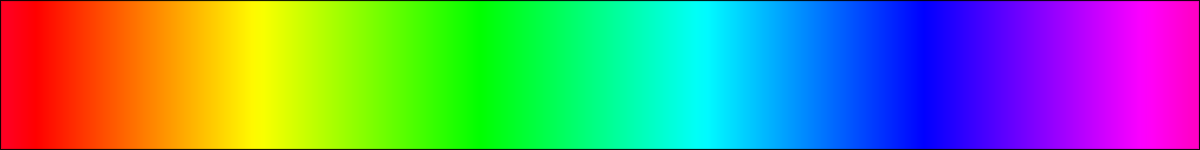
\includegraphics[width = 4.25cm, height = .3cm]{\here/colorbars/rb.png}};

\begin{groupplot}[
		group style = {
			group size = 3 by 1,
			vertical sep = .25cm,
			horizontal sep = .1cm, 
			},
		width = 4.25cm,
		height = 4cm,
		enlargelimits = 0.05,
		simpleax1,
		% ytick = {0,50},
		xticklabel = \empty,
		% xmin = 0.5,
		% xmax = 10.5,
		ymin = 0,
		ymax = 5.5,
		ytick pos = right, 
		yticklabel pos = right,
		scale only axis,
		enlargelimits = false,
		% xtick = {1.5,...,10.5},
		legend style = {
			at = {(0.5,1)},
			anchor = south,
			legend1},
		legend columns = 3,
		xtick = \empty,
		]


		\nextgroupplot[ymax = 100, ylabel = \empty, yticklabel = \empty]
		\addplot[ultra thick, hcqred]table[]{cmap_analytics/rb_L.txt};

		\nextgroupplot[xshift = .9cm, ylabel = \empty, yticklabel = \empty]
		\addplot[ultra thick, hcqred]table[y index = 1]{cmap_analytics/rb_d.txt};
		
		% \addlegendentry{$\Delta E^*_{ab}$}
		% \addlegendentry{$\Delta E^*_{2000}$}
		% \addlegendimage{hcqblue, ultra thick, mark = triangle*, mark options = {thin, fill = hcqblue, draw = black}};
		% \addlegendentry{$L$};
		

		\nextgroupplot[ylabel = \empty, yticklabel = \empty, ymax = 100, ytick pos = right, yticklabel pos = right]
		\addplot[hcqred, ultra thick]table[]{cmap_analytics/rb_d_cum.txt};
		% \addplot+[hcqred, ultra thick, mark options = {thin, fill = hcqred, draw = black}]table[y index = 2]{coldiff2000.txt};

		% \addlegendentry{$\Delta E^*_{ab}$}
		% \addlegendentry{$\Delta E^*_{2000}$}
		% \addlegendimage{hcqblue, ultra thick, mark = triangle*, mark options = {thin, fill = hcqblue, draw = black}};
		% \addlegendentry{$L$};


		% \nextgroupplot[]
		% \addplot+[hcqyellow, ultra thick, mark options = {thin, fill = hcqyellow, draw = black}]table[y index = 3]{coldiffLab.txt};
		% \addplot+[hcqred, ultra thick, mark options = {thin, fill = hcqred, draw = black}]table[y index = 3]{coldiff2000.txt};


		% \addlegendentry{$\Delta E^*_{ab}$}
		% \addlegendentry{$\Delta E^*_{2000}$}
		% \addlegendimage{hcqblue, ultra thick, mark = triangle*, mark options = {thin, fill = hcqblue, draw = black}};
		% \addlegendentry{$L$};

	\end{groupplot}

	\node[text width=1em, anchor=west]at(group1 c1r1.north west){\subcaptionbox{\label{cmA}}{}};
	\node[text width=1em, anchor=west]at(group1 c2r1.north west){\subcaptionbox{\label{cmB}}{}};
	\node[text width=1em, anchor=west]at(group1 c3r1.north west){\subcaptionbox{\label{cmC}}{}};
\end{tikzpicture}

% 	\caption{Note: Scales are not directly comparable! But shape of each individual line is what matters here.}
% 	\label{fig:cmapanalytics}
% \end{figure}



% Here is how you define a new ColorScheme:
% \begin{listing}[h]
% \begin{minted}[xleftmargin = 1.5cm]{julia} 
% using Colors, ColorSchemes
% cividis_cols = ColorSchemes.cividis.colors
% cividis_protanopic = ColorScheme(protanopic.(cividis_cols, 1))
% \end{minted}
% \end{listing}



% \begin{tikzpicture} 
% 	\begin{groupplot}[
% 		group style = {
% 			group name = name1,
% 			group size = 2 by 1,
% 			vertical sep = 1cm,
% 			horizontal sep = 1cm, 
% 			},
% 			view={0}{90},
% 			simpleax1,
% 		]
	
% 		\nextgroupplot[colormap/jet, colorbar horizontal]
% 		% \addplot3[surfstyle, samples = 500, domain = 0:7, y domain = 0:1]{(1 - y) * cos(deg(x)*cos(deg(x)))}; 
% 		\addplot3[surfstyle, samples = 500, domain = 0:7, y domain = 0:1]{cos(deg(x))}; 
		 
% 		% \nextgroupplot[colormap/viridis, colorbar horizontal] 
% 		% \addplot3[surfstyle]{cos(deg(y)) + cos(deg(x))}; 
	
% 	\end{groupplot} 
% \end{tikzpicture}



% Why is viridis a good color map? Perceptional 



% Describe example...

% Main message: Human perception does not linearly 
% .
% What we actually want is that colors that are equally apart in our colormap are also perceived by the human eye / brain as equally apart.
% The $\Delta E$ we are looking for is actually the difference in the perception! to define such a dE, one needs to know a lot about how the eye/brean mechanism of color perception works one has to work with real humans! That goes back to the 30. One can come up with a good measure, has been refined, etc.
%  Let us see how our three colormaps perform agains this metric.



% Besides being colorblind-friendly, the most reasonable claim is that the distance between 



% \section{Know the enemy: An example of a really bad colormap}\label{sec:rainbow}



% A colormap is a one-dimensional subspace of 



% There are plenty of different color spa





% perceptually uniform colorspaces are and why you should be using them:
% Unfortunately many widely used colour maps 1 provided by vendors have
% highly uneven perceptual contrast. Colour maps may have points of locally
% high colour contrast leading to the perception of false anomalies in your data
% when there is none. Conversely colour maps may also have ‘flat spots’ of
% low perceptual contrast that prevent you from seeing features in the data.




% Perceptual uniformity: Same distance in color (difficult! Has to do with color perception, i.e. human vision), same distance in space. 
% Not colorblind safe.
% Not same order!
% Mach bands!


\section{Summary}

				% Regular chapter
	\chapter{Bibliography with BibLaTeX}\label{cha:biblatex}			% Regular chapter
	\chapter{General remarks}\label{cha:remarks}

use newcommands for ...
read the promotionsordnung
whatever you do, do it consistently
In case of trouble, first step is to delete cached files

\section{Define your own commands}
\verb|\figref|
			% Regular chapter

	\tikzexternaldisable
	\chapterimage
	\part{Example part page}\label{part:examplepartpage}

	\bookmarksetup{startatroot} % Fix pdf toc hierarchy
	\chapter{Test chapter}

	\appendix
	\chapter{Appendix for Chapter 1}
\section{blabsnhfsdfsdf}
\subsection{Subsection in Appendix}
\subsubsection{Subsubsection}
Don't use! Looks weird.
\paragraph{Paragraphs} look much better.	% Appendix chapter

	%%%%%%%%%%%%%%%%%%%% Bibliography %%%%%%%%%%%%%%%%%%%%
	
	\cleardoublepage
	\phantomsection	% For correct hyperlink	
	\addcontentsline{toc}{chapter}{Bibliography}

	% Print my own papers with prefix P (= paper / published) and my name in bold.
	\boldname{Berke}{Christoph}{C.}
	\newrefcontext[labelprefix=P]
	\printbibliography[category=own]

	% Print unpublished papers with prefix U
	\newrefcontext[labelprefix=U]
	\printbibliography[category=prep, heading=none,]

	% Print all other papers
	\newrefcontext[labelprefix=]
	\printbibliography[notcategory=own,notcategory=prep,heading=none,resetnumbers=true]


	%%%%%%%%%%%%%% Acknowledgements + Erklaerung %%%%%%%%%%%%%%%%%
	% Erklaerung

\cleardoublepage
\thispagestyle{empty}

% Add toc to pdfreader content but not to toc.
\phantomsection
\pdfbookmark{Acknowledgements}{asd}

\begin{center}
{\color{accentcolor2} \mainregular \Huge Acknowledgements} 
\end{center}
\vspace{1cm}

Since I forgot to mention them in the acknowledgments of my thesis, it's probably about time to thank all the incredible contributors on TeX.StackExchange who tirelessly help others solve their problems. I have particularly benefited from the insights and solutions provided by egreg, David Carlisle, Ulrike Fischer, Gonzalo Medina, Heiko Oberdiek, Martin Scharrer, Stefan Kottwitz, Lockstep, Jake, Peter Grill, Alan Munn, samcarter\_is\_at\_topanswers.xyz, Moewe, Percusse, Christian Feuersänger, Stefan Pinnow, and many others. Your expertise and generosity are truly appreciated!
	\cleardoublepage
\thispagestyle{empty}
\pdfbookmark{Erkl\"arung}{erklaerung}

\begin{center}
{\color{maincolor2} \mainregular \Huge Erkl\"arung} 
\end{center}
\vspace{1cm}

\noindent Hiermit versichere ich an Eides statt, dass ich die vorliegende Dissertation selbstst\"andig und ohne die Benutzung anderer als der angegebenen Hilfsmittel und Literatur angefertigt habe. Alle Stellen, die w\"ortlich oder sinngem\"a\ss~aus ver\"offentlichten und nicht ver\"offentlichten Werken dem Wortlaut oder dem Sinn nach entnommen wurden, sind als solche kenntlich gemacht. Ich versichere an Eides statt, dass diese Dissertation noch keiner anderen Fakult\"at oder Universit\"at zur Pr\"ufung vorgelegen hat; dass sie -- abgesehen von unten angegebenen Teilpublikationen und eingebundenen Artikeln und Manuskripten -- noch nicht ver\"offentlicht worden ist sowie, dass ich eine Ver\"offentlichung der Dissertation vor Abschluss der Promotion nicht ohne Genehmigung des Promotionsausschusses vornehmen werde. Die Bestimmungen dieser Ordnung sind mir bekannt. Dar\"uber hinaus erkl\"are ich hiermit, dass ich die Ordnung zur Sicherung guter wissenschaftlicher Praxis und zum Umgang mit wissenschaftlichem Fehlverhalten der Universit\"at zu K\"oln gelesen und sie bei der Durchf\"uhrung der Dissertation zugrundeliegenden Arbeiten und der schriftlich verfassten Dissertation beachtet habe und verpflichte mich hiermit, die dort genannten Vorgaben bei allen wissenschaftlichen T\"atigkeiten zu beachten und umzusetzen. Ich versichere, dass die eingereichte elektronische Fassung der eingereichten Druckfassung vollst\"andig entspricht.
\vspace{0.5cm}

\begin{center}
\noindent {\color{maincolor2} \mainregular \normalsize Teilpublikationen:} \\
(bereits ver\"offentlicht)
\end{center}

\boldname{Berke}{Christoph}{C.}
\newrefcontext[labelprefix=P]
\printbibliography[category=own,heading=none]

\begin{center}
(in Vorbereitung)
\end{center}

\boldname{Berke}{Christoph}{C.}
\newrefcontext[labelprefix=U]
\printbibliography[category=prep,heading=none]

\vspace{1.5cm}

\noindent K\"oln, den xx. Monat xxxx \hfill
\begin{minipage}[t]{4.5cm}\begin{center}
	\rule[-1pt]{4cm}{.4pt}\vskip -5pt
	{\scriptsize (Your Name)}
\end{center}
\end{minipage}


\end{document} 

